%%%%%%%%%%%%%%%%%%%%%%%%%%%%%%%%%%%%%%%%%%%%%%%%%%%%%%%%%
\setcounter{equation}{0}
\section{The kernel as a Fourier sum: Proof of \texorpdfstring{\cref{prop:perfect_recon}}{Proposition 5.1}}
\label{app:perfect_recon}
We now turn to proving how we can rewrite a translation-invariant kernel map in terms of a Fourier transform. To recall, our claim is that:

{
% \settheoremtag{\ref{prop:perfect_recon} again}
\begin{proposition*}[Perfect reconstruction of kernel] % was proposition*
  For any periodic, translation-invariant, symmetric, positive definite kernel $\tk$ as defined in \cref{eq:krnl_approx},
  we have $\forall\, \tx',\tx\in\tsX$
  \begin{align*}
    \tk\left(\tx',\tx\right) &= \frac{1}{G^D} \sum_{\tv\in\tsV}Q^{\tau}(\tv)\overline{\varphi(\tv,\tx')}\varphi(\tv,\tx)\nonumber\\
                            &=\Braket{\tx'|\F_{D}^\dag \Q^{\tau} \F_{D}|\tx}.
  \end{align*}
\end{proposition*}
}

\begin{proof}
  To begin, recall that any translation-invariant kernel $k:\sX\times\sX\to\R$ can be written as
  \begin{equation*}
    \tag{I'm \ref{eq:kernel_as_exp_of_features}}
    k(x',x)=k\left(x'-x\right)=\int_\sV d\tau(v)\overline{\varphi\left(v,x'\right)}\varphi\left(v,x\right),
  \end{equation*}
  where \cref{eq:varphi_defn} defines $\varphi(v,x):=\ee^{-2\pi\ii v\cdot x}$, and the density function
  \begin{equation*}
    \tag{I'm \ref{eq:q-tau-as-Fourier-k}}
    q^{\tau}(v)=\int_\sX dx\,\ee^{-2\pi\ii v\cdot x}\,k(x)
  \end{equation*}
  is the Fourier transform of the kernel.
  Also recall that we approximate $k(x',x)$ by
  \begin{equation*}
    \tag{I'm \ref{eq:krnl_approx}}
    \tk(x',x):=\sum_{n\in\Z^D}k(x',x+Gn),
  \end{equation*}
  whence $\tk$ inherits the translation invariance of $k$, in addition to being periodic; in particular $\forall\, n'\in\Z^D$ 
  \begin{align*}
    \label{eq:periodicity}
    \tk(x'+Gn',x)&=\sum_{n\in\Z^D}k(x'+Gn',x+Gn)\\
                &=\sum_{n\in\Z^D}k(x'+Gn'-x-Gn) \\ % \tag*{(translation-invariance)}
                &=\sum_{n\in\Z^D}k(x',x+G(n-n'))\\
                &=\tk(x',x),
  \end{align*}
where the second line uses the translation invariance of $k$.

Shannon's sampling theorem~\cite{Shannon1949communication,proakis2001digital} is used in signal processing to show that we can perfectly reconstruct any one-dimensional kernel function $\tk$ on a \textit{continuous} domain $I=\left[-\frac{G}{2},\frac{G}{2}\right]$ using a \textit{discrete} set of frequencies from its Fourier transform. The Fourier transform of a $1$D kernel on $I$ is given by
\begin{align}
  \int_{-\frac{G}{2}}^{\frac{G}{2}}dx\,\ee^{-2\pi\ii vx}\, \tk(x)
            &=\int_{-\infty}^{\infty}dx\,\ee^{-2\pi\ii vx}\, k(x) \nonumber\\
            &=q^{\tau}(v).
\end{align}
The inverse Fourier transform then allows us to reconstruct $\tk$ from $q^\tau$
\[
  \tk(x) = \int_{-\infty}^{\infty}dv\,\ee^{2\pi\ii vx}\, q^{\tau}(v).
\]
The sampling theorem says that $\forall\, x\in I$, using only discrete frequencies $v\in\Z$ we can still recover $\tk$ exactly, i.e.\
\begin{equation}
  \label{seq:one_dim}
  \tk(x)=\frac{1}{G}\sum_{v=-\infty}^{\infty}q^{\tau}\left(\nicefrac{v}{G}\right)\ee^{\nicefrac{2\pi\ii v x}{G}}.
\end{equation}
Furthermore, since $\tk(x)$ is periodic, the above equality actually holds for any $x\in\R$.
Analogously, for any $D\geq 1$, we have $\forall\, x\in\R^D$
\begin{equation}
  \label{seq:D_dim}
  \tk(x)=\frac{1}{{G}^D}\sum_{v\in\Z^D}q^{\tau}\left(\nicefrac{v}{G}\right)\ee^{\nicefrac{2\pi\ii v\cdot x}{G}}.
\end{equation}

\parahead{From $\Z^D$ to $\tsX$:} Since our data domain 
\(
  \tsX=\left\{0,1,\ldots,{G}-1\right\}^D
\) is actually \textit{discretised} and finite,
$\tk(x)$ can be perfectly reconstructed on $\tsX$ via the $D$-dimensional DFT, using only a \textit{finite} set of discrete frequency modes. As in the recipe for the sampling theorem, first consider the DFT of $\tk$
\begin{align}
  \label{eq:discrete_Fourier}
  \left(\mathrm{DFT}\,\tk\right)(\tx)
          &=\frac{1}{\sqrt{{G}^D}}\sum_{\tx'\in\tsX}\tk(\tx')\ee^{\nicefrac{-2\pi\ii \tx'\cdot \tx}{G}}\nonumber\\
          &=\frac{1}{\sqrt{{G}^D}}\sum_{\tx'\in\tsX}\left(\frac{1}{{G}^D}\sum_{v'\in\Z^D}q^{\tau}\left(\nicefrac{v'}{G}\right)\ee^{\nicefrac{2\pi\ii  v'\cdot \tx'}{G}}\right)\ee^{\nicefrac{-2\pi\ii \tx'\cdot \tx}{G}}\nonumber\\
          &=\frac{1}{\sqrt{{G}^D}}\sum_{v\in\Z^D}q^{\tau}\left(\frac{\tx}{G}+v\right),
\end{align}
since the sum over $\tx'$ in the second line is nonzero iff $ v'=\tx+Gv$ for $v\in\Z^D$. Denoting $\nicefrac{\tx}{G}$ by $\tv$, we are thus lead naturally to the definition \cref{eq:Q-tau} of $Q^{\tau}:\tsV \to\R$
\begin{equation}
  \label{eq:q_tau_g_function}
  Q^{\tau}(\tv):=\sum_{v\in\Z^D}q^{\tau}\left(\tv+v\right),
\end{equation}
where $\tsV $ is the finite set  of features
\begin{equation*}
      \tag{I'm \ref{eq:finite_feature_set}}
      \tsV :={\left\{0,\frac{1}{G},\ldots,1-\frac{1}{G}\right\}}^D,
\end{equation*}
and the bijection $\tv\mapsto G\tv$ lets us go back and forth between $\tsV $ and $\tsX$.

Finally, inverting the  DFT of~\cref{eq:discrete_Fourier},
we obtain $\forall \tx',\tx\in\tsX$ the perfect reconstruction of the kernel $\tk(\tx',\tx)$ using the feature points in $\tsV $ and the function $Q^{\tau}$
\begin{align}
  \label{eq:perfect_reconstruction}
  \tk\left(\tx',\tx\right)&=\tk\left(\tx'-\tx\right)\nonumber\\
  &=\frac{1}{{G}^D}\sum_{\tv\in\tsV} Q^{\tau}(\tv)\, \ee^{2\pi\ii \tv\cdot \left(\tx'-\tx\right)}\nonumber\\
  &=\frac{1}{{G}^D}\sum_{\tv\in\tsV }Q^{\tau}(\tv)\overline{\varphi\left(\tv,\tx'\right)}\varphi\left(\tv,\tx\right),
\end{align}

To put this in matrix form, we defined in \cref{eq:q_tau_g} the diagonal operator
\begin{align*}
  \Q^{\tau}&:=\sum_{\tv\in\tsV}Q^{\tau}(\tv)\ketbra{\tv}\nonumber\\
          &\equiv\sum_{\tx\in\tsX}Q^{\tau}\left(\nicefrac{\tx}{G}\right)\ketbra{\tx}
\end{align*}
corresponding to $Q^{\tau}(\tv)$. Denote by $\F$ the one-dimensional DFT on $\Z_{G}$, with matrix elements
\begin{align*}
  \F_{\tx',\tx} := \frac{1}{\sqrt{{G}}}\,\omega^{-\tx'\tx},
\end{align*}
written in terms of the $G^{th}$ root of unity 
\begin{equation*}
  \omega = \ee^{\nicefrac{2\pi\ii}{G}}.
\end{equation*}
$\F_{D} := \F^{\otimes D}$ is then the $D$-dimensional DFT on $(\Z_G)^{\times D}$, with matrix entries
\begin{equation}
  \label{eq:F_D}
  \left(\F_{D}\right)_{\tx',\tx} := \frac{1}{\sqrt{{G^D}}}\,\omega^{-\tx'\cdot\tx}.
\end{equation}
These matrix entries are values of the feature map $\varphi:\sV\times\sX\to\C$ evaluated on $\tsV\times\tsX$, i.e.\
\begin{align}
  \label{eq:feature}
  \varphi\left(\tv,\tx\right) = \ee^{-2\pi\ii \tv\cdot\tx}
                              &=\sqrt{{G}^D}\Braket{\tv|\F_{D}|\tx} \nonumber\\
                              &=\sqrt{{G}^D}\Braket{\tx|\F_{D}|\tv}.
\end{align}
The second line captures the invariance of $\F_{D}$ under transpose with respect to the computational basis.
From \cref{eq:perfect_reconstruction,eq:F_D,eq:feature}, we finally have $\forall\, \tx',\tx\in\tsX$
\begin{equation}
  \label{eq:kernel_decomposition}
  \tk\left(\tx',\tx\right)=\Braket{\tx'|\F_{D}^\dag \Q^{\tau} \F_{D}|\tx}.
\end{equation}
\end{proof}

%%%%%%%%%%%%%%%%%%%%%%%%%%%%%%
\subsection*{Which kernels can we use?}
\label{app:which_kernels}

Our quantum algorithm can use any translation-invariant kernel $\tk$ in the form of its perfect reconstruction, \cref{prop:perfect_recon}. However, speedups may only be possible in some parameter regimes, and to this end we sneak in some additional (mild) assumptions below.

$Q^{\tau}(\tv)$ ought to be a classically efficiently computable, in time at most $\O(\poly(D))$ time.
We also assume efficient precomputation of its maximum,
\begin{equation*}
  \tag{I'm \ref{eq:q_tau_g_max}}
  {Q_{\max}^{\tau}}:=\max\big\{Q^{\tau}(\tv):\tv\in\tsV\big\}.
\end{equation*}
We further assume that the kernel's parameters can be adjusted appropriately to ensure $\tk(0,0)=\Omega(1)$, and that $q^\tau$ has no pathological peaks, so that $Q_{\max}^{\tau}=\O(\poly(D)))$.

\begin{remark*}
  As touched upon in \cref{featureSamp:perfect_reconstruction}, let $P^{\tau}$ be the normalised probability mass function induced by $Q^{\tau}$ on $\tsV$ 
  \begin{equation}
    \label{eq:normalisation_p_tau}
    P^{\tau}(\tv) := \frac{Q^{\tau}(\tv)}{\displaystyle\sum_{\tv'\in\tsV}Q^{\tau}(\tv')}.
  \end{equation}
  We obtain from~\cref{eq:perfect_reconstruction}
  \begin{equation}
    \tk(0,0)=\frac{1}{{G}^{D}}\sum_{\tv\in\tsV }Q^{\tau}(\tv),
  \end{equation}
  and hence, we can regard $\tk(0,0)$ as the normalisation factor in
  \begin{equation}
    P^{\tau}(\tv)=\frac{1}{\tk(0,0)} \frac{Q^{\tau}(\tv)}{G^D}.
  \end{equation}
  This yields a lower bound on the maximum value of $Q^{\tau}$ (cf. \eqref{eq:q_tau_g_max})
  \begin{equation}
    Q_{\max}^{\tau}=G^D\times\frac{Q_{\max}^{\tau}}{G^D}\geq \sum_{\tv\in\tsV}\frac{Q^{\tau}(\tv)}{G^D}=\tk(0,0).
  \end{equation}
  \end{remark*}
  

With $Q^{\tau}$ precomputed\footnote{$\Or_\tau$ can then be efficiently implemented with either quantum arithmetics, or QRAM and a lookup table.}, we quantumly access it where needed with an oracle $\Or_\tau$
\begin{equation}
  \label{eq:oracle_tau_definition}
\Or_\tau~\Ket{v}\Ket{0} = \ket{v}\ket{Q^{\tau}(v)},
\end{equation}
and denote its runtime $T_\tau$ per query. In fact, in practice many important cases of $Q^{\tau}$ are classically efficiently computable, so that we can have an efficient subroutine that efficiently computes $Q^{\tau}(v)$ on the fly as and when needed. We assume $Q^{\tau}(v)\in\R$ is computed to sufficient precision, and omit the overheads, which only contribute weak logarithmic factors to the runtime and ancillary qubit requirement.

%%%%%%%%%%%%%%%%%%%%%%%%%%%%%%%%%%%%%%%%%%%%%%%%%%%%%
\begin{table}[htb]
  \begin{center}
  \renewcommand{\arraystretch}{1.7}
  \begin{tabular}{|l|c|c|c|}
  \toprule
  & $k(x',x)$ & $Q^{\tau}(\tv)$ & $\tk(0,0)$ \\
  \midrule
  Gaussian & $\exp\left(-\gamma\left\|x'-x\right\|_2^2\right)$ & $\displaystyle\prod_{i=1}^D\vartheta\left(\pi \tv^i;e^{-\gamma}\right)$ & $\displaystyle\frac{1}{1-\ee^{-\gamma}}\geq 1$\\
  Laplacian & $\exp\left(-\gamma\left\|x'-x\right\|_1\right)$ & $\displaystyle\prod_{i=1}^D\frac{\sinh\left(\gamma\right)}{\cosh\left(\gamma\right)-\cos\left(2\pi \tv^i\right)}$ & $''$\\
  \bottomrule
  \end{tabular}
  \end{center}
  \caption{Examples of the distribution function $Q^{\tau}(\tv)$ for typical kernels. $\tv={(\tv^1,\ldots,\tv^D)}^\mathrm{T}$, and $\vartheta$ is the theta function
  $\vartheta\left(u;q\right):= 1+2\sum_{n=1}^{\infty}q^{n^2}\cos\left(2nu\right)$.}
  \label{table:kernel}
  \end{table}
  %%%%%%%%%%%%%%%%%%%%%%%%%%%%%%%%%%%%%%%%%%%%%%%%%%%%%

\begin{remark*}
  \cref{table:kernel} illustrates that representative choices of kernels, such as the Gaussian and Laplacian, satisfy our assumptions. For these kernels, $Q^{\tau}$ is a product of $D$ special functions, computable classically in time $T_\tau=\O(D)$.
  Also, $Q_{\max}^{\tau}=Q^{\tau}\left(0\right)$, and can be made $\O\left(\poly\left(D\right)\right)$ by reducing the parameter $\gamma>0$. In fact, decreasing $\gamma$ enlarges the class of learnable functions.
  These examples indicate that the assumptions made in this section are weak and easy to satisfy.
  We reiterate that our algorithm \textit{does not} impose sparsity or low rank on $\krn$ or $\hbq^{\rho}$,
  making it more widely applicable than previous QML algorithms.
\end{remark*}


%%%%%%%%%%%%%%%%%%%%%%%%%%%%%%%%%%%%%%%%%%%%%%%%%%%%%%%%%%%%%%%%%%%%%%%%%%%%%%%%%%%%%%%%%%%%%%%%%%%%%%%%%%%%%%%%%%
\setcounter{equation}{0}
\section{The state that encodes \texorpdfstring{$Q^*P$}{Q\textsuperscript{*}P}: Proof of \texorpdfstring{\cref{prop:state}}{Proposition 5.2}}
\label{app:featureSamp_state}

% {
% % \settheoremtag{\ref{prop:state} again}
% \begin{proposition*}[Quantum state for sampling an optimised random feature]

  We had claimed that the bipartite quantum state 
  \begin{equation}
    \label{eq:state}
    \Ket{\Psi}\propto\sum_{\tv\in\tsX}\hSgOp_{\epsilon}^{-\frac{1}{2}}\Ket{\tv}^X\otimes \sqrt{\uQ^{\tau}}\F_D^\dag\sqrt{\hbq^{\rho}}\Ket{\tv}^{X'}
  \end{equation}
  defined on two registers $X$ and $X'$ of $\lceil D\log G\rceil$ qubits each is our means to sampling optimised random features. In particular, 
  measuring the register $X'$ of $\Ket{\Psi}$ in the computational basis $\{\Ket{\tv}^{X'}:\tv\in\tsV\}$, we obtain a measurement outcome $\tv$ with probability 
  \begin{align}
    \label{eq:pr-v-app-state}
    \Pr(\tv) &= Q_{\epsilon}^\ast(\tv)P^{\tau}(\tv).
             % &=Q_{\epsilon}^\ast\left(\frac{\tx}{{G}}\right)P^{\tau}\left(\frac{\tx}{{G}}\right).
  \end{align}

  % \end{proposition*}
% }

% \begin{proof}

  Recall \cref{eq:p-tau-defn} and the definition of the optimised probability distribution $Q_{\epsilon}^\ast(\tv)P^{\tau}(\tv)$
  \begin{equation}
    \label{eq:state_1}
    Q_{\epsilon}^\ast(\tv)P^{\tau}(\tv)=
    \frac{1}{\Gamma}Q^{\tau}(\tv)\Braket{\varphi\left(\tv,\cdot\right) | \hbq^{\rho}{\left({\hSgOp}+\epsilon\id\right)}^{-1} | \varphi\left(\tv,\cdot\right)},
  \end{equation}
  where the normalisation factor is just
  \begin{equation}
    \label{eq:gamma-normalisation}
    \Gamma = \sum_{\tv'\in\tsV }Q^{\tau}(\tv')\Braket{\varphi\left(\tv',\cdot\right) | \hbq^{\rho}{\left({\hSgOp}+\epsilon\id\right)}^{-1} | \varphi\left(\tv',\cdot\right)}.
  \end{equation}

  $\hSgOp=\krn \hbq^{\rho}$ is the empirical integral operator, with the discretised kernel matrix and empirical data density given by (\cref{{featureSamp:data}})
  \begin{align*}
    \krn \quad &= \quad \sum_{\tx',\tx\in\tsX}\tk\left(\tx',\tx\right)\Ket{\tx'}\Bra{\tx},\\
    \hbq^{\rho} \quad &=\quad \sum_{\tx\in\tsX}\hq^{\rho}(\tx)\Ket{\tx}\Bra{\tx},
  \end{align*}
  and we will interchangeably interpret the ket labels as $\tv\in\tsV$ or the corresponding $\tx=G\tv\in\tsX$.
Since functions become vectors under discretisation (\cref{table:coarse_graining}), using \cref{eq:feature} we have
\begin{align*}
  \Ket{\varphi\left(\tv,\cdot\right)} &= \frac{1}{\sqrt{{G}^D}}\sum_{\tx\in\tsX}\varphi\left(\tv,\tx\right)\ket{\tx}\\
                                      &= \sum_{\tx\in\tsX}\left(\F_D\right)_{\tv,\tx}\ket{\tx}\\
                                      &= \F_{D}\Ket{\tv},
\end{align*}
exploiting the symmetry $\F_D^\mathrm{T}=\F_D$ enjoyed by the QFT (DFT) in the computational basis, and as usual, using the equivalence of the two finite sets $\tsV$ and $\tsX$. 

  Then, we have
  \begin{align}
    \label{eq:state_2}
    \Pr(\tv)
    &=\frac{1}{\Gamma}Q^{\tau}(\tv)\Braket{\varphi\left(\tv,\cdot\right) | \hbq^{\rho}{\left({\hSgOp}+\epsilon\id\right)}^{-1} | \varphi\left(\tv,\cdot\right)} \nonumber\\
    &=\frac{1}{\Gamma}Q^{\tau}(\tv)\Braket{\tv|\F_{D}^\dag \hbq^{\rho}{\left({\hSgOp}+\epsilon\id\right)}^{-1} \F_{D} | \tv}.
  \end{align}
  Then, plugging in $\Q^{\tau}$ from \cref{eq:q_tau_g}, we obtain
  \begin{equation}
    \Pr(\tv)
      =\frac{1}{\Gamma}\Braket{\tv|\sqrt{\Q^{\tau}}\F_{D}^\dag \hbq^{\rho}{\left({\hSgOp}+\epsilon\id\right)}^{-1} \F_{D} \sqrt{\Q^{\tau}}| \tv}.
  \end{equation}
  Multiplying and dividing by $Q_{\max}^{\tau}$, we can manipulate this into the form
  \begin{align}
    \label{eq:hat_p_lambda}
    \Pr(\tv)
    &=\frac{1}{\Gamma}{\Braket{\tv|\sqrt{\uQ^{\tau}}\F_{D}^\dag \hbq^{\rho}{\left[\frac{1}{Q_{\max}^{\tau}}\left(\hSgOp+\epsilon\id\right)\right]}^{-1} \F_{D} \sqrt{\uQ^{\tau}}| \tv}},
  \end{align} % 
where we denote $\Q^{\tau}$ normalised by $Q_{\max}^{\tau}$ as
\begin{equation*}
  \tag{I'm \ref{eq:Q-by-Q-max-notation}}
  \uQ^{\tau} := \frac{1}{Q_{\max}^{\tau}}\Q^{\tau}
\end{equation*}
to keep the notation manageable. We had previously defined in \cref{sec:featureSamp_state} a positive definite operator with full support on $\sH^X$
\begin{equation*}
  \tag{I'm \ref{eq:sigma-epsilon-full-rank}}
  \hSgOp_\epsilon:=\frac{1}{Q_{\max}^{\tau}}\left(\sqrt{\hbq^{\rho}}\krn\sqrt{\hbq^{\rho}}+\epsilon\id\right).
\end{equation*} Since $\hbq^{\rho}$ may not have full rank, we define on the support of $\q^{\rho}$ the corresponding operator 
\begin{align*}
  \hSgOp_\epsilon^{\rho}&:= \frac{1}{Q_{\max}^{\tau}} \cdot \sqrt{\hbq^{\rho}}\left(\hSgOp+\epsilon\id\right){\left(\hbq^{\rho}\right)}^{-\frac{1}{2}}\nonumber\\
                                    &=\frac{1}{Q_{\max}^{\tau}}\left(\sqrt{\hbq^{\rho}}\krn\sqrt{\hbq^{\rho}}+\epsilon\Pi^{\rho}\right) % \tag{since $\hSgOp=\krn\hbq^\rho$},
\end{align*}
where ${\left(\hbq^{\rho}\right)}^{-\frac{1}{2}}$ denotes the square root of the Moore-Penrose pseudoinverse of $\hbq^{\rho}$, and $\Pi^{\rho}$ projects onto the support of $\q^{\rho}$. Clearly, $\hSgOp_\epsilon^{\rho}=\Pi^{\rho}\hSgOp_\epsilon\Pi^{\rho}$, and since $\krn$ is a symmetric matrix in the computational basis, both $\hSgOp_\epsilon$ and $\hSgOp_\epsilon^{\rho}$ are also symmetric.

We have by definition
\begin{equation}
  {\left(\hSgOp_\epsilon^{\rho}\right)}^{-1} = {\left(\hbq^{\rho}\right)}^{\frac{1}{2}}{\left[\frac{1}{Q_{\max}^{\tau}}\left({\hSgOp}+\epsilon\id\right)\right]}^{-1}{\left(\hbq^{\rho}\right)}^{-\frac{1}{2}}.
\end{equation}

We can now proceed to further simplify \cref{eq:hat_p_lambda}:
\begin{align}
  \label{eq:p_lambda_ast_simplified}
  \Pr(\tv)
  &=\frac{1}{\Gamma}{\Braket{\tv|\sqrt{\uQ^{\tau}}\F_{D}^\dag \sqrt{\hbq^{\rho}}{\left(\hSgOp_\epsilon^{\rho}\right)}^{-1} \sqrt{\hbq^{\rho}} \F_{D} \sqrt{\uQ^{\tau}}| \tv}}\nonumber\\
  &=\frac{1}{\Gamma}{\Braket{\tv|\sqrt{\uQ^{\tau}}\F_{D}^\dag \sqrt{\hbq^{\rho}}\hSgOp_\epsilon^{-1} \sqrt{\hbq^{\rho}} \F_{D} \sqrt{\uQ^{\tau}}| \tv}},
  % \tag{{\small since $\Pi^\rho\sqrt{\hbq^{\rho}}=\sqrt{\hbq^{\rho}}$, \& $\left(\hSgOp_\epsilon^{\rho}\right)^{-1}=\left(\hSgOp_\epsilon\right)^{-1}\Pi^{\rho}$, by definition of $\Pi^\rho$}}
\end{align}
since $\Pi^\rho\sqrt{\hbq^{\rho}}=\sqrt{\hbq^{\rho}}$, and $\left(\hSgOp_\epsilon^{\rho}\right)^{-1}=\Pi^{\rho}\left(\hSgOp_\epsilon\right)^{-1}\Pi^{\rho}$, by definition of $\Pi^\rho$.

% where this probability distribution is normalised by 
% \[
%   \sum_{\tx\in\tsX}Q_{\epsilon}^* \left(\frac{\tx}{G}\right) P^{\tau}\left(\frac{\tx}{G}\right)=1.
% \]

Let us now turn our attention to the quantum state in \cref{eq:state}. For any two operators $A$ on $\sH^X$ and $B$ on $\sH^{X'}$, where $\dim\sH^X=\dim\sH^{X'}$, we have what is often called the `transpose trick'~\cite{Nielsen2010}
\begin{equation}
  \sum_{x\in X}A\Ket{x}^X\otimes B\Ket{x}^{X'}=\sum_{x\in X}\Ket{x}^X\otimes BA^\mathrm{T}\Ket{x}^{X'},
\end{equation}
a property that is extensively exploited in manipulations of maximally entangled bipartite states, and the Choi-Jamio{\l}kowski isomorphism.
Applying this to~\cref{eq:state}, 
\begin{align}
  \Ket{\Psi}&\propto\sum_{\tv\in\tsV}\hSgOp_\epsilon^{-\frac{1}{2}}\Ket{\tv}^X\otimes \sqrt{\uQ^{\tau}}\F_{D}^\dag\sqrt{\hbq^{\rho}}\Ket{\tv}^{X'}\nonumber\\
  &=\sum_{\tv\in\tsV}\Ket{\tv}^X\otimes \sqrt{\uQ^{\tau}}\F_{D}^\dag\sqrt{\hbq^{\rho}}\hSgOp_\epsilon^{-\frac{1}{2}}\Ket{\tv}^{X'},
\end{align}
using the symmetry of $\hSgOp_\epsilon$.
If we measure $\Ket{\Psi}$ in the computational basis $\left\{\ket{\tv}^X\otimes\ket{\tv'}^{X'}\right\}$, the probability distribution of measurement outcomes is
\begin{align}
  p(\tv,\tv')&=\left|\left(\bra{\tv}^X\otimes\bra{\tv'}^{X'}\right)\Ket{\Psi}\right|^2\nonumber\\
               &\propto\left|\Braket{\tv'|\sqrt{\uQ^{\tau}}\F_{D}^\dag\sqrt{\hbq^{\rho}}\hSgOp_\epsilon^{-\frac{1}{2}}|{\tv}}\right|^2\nonumber\\
               &=\Braket{\tv'|\sqrt{\uQ^{\tau}}\F_{D}^\dag\sqrt{\hbq^{\rho}}\hSgOp_\epsilon^{-\frac{1}{2}}|\tv}\Braket{\tv|\hSgOp_\epsilon^{-\frac{1}{2}}\sqrt{\hbq^{\rho}}\F_{D}\sqrt{\uQ^{\tau}}|\tv'}.
\end{align}
Measuring the register $X'$ alone yields an outcome $\tv'$ with probability given by tracing out the register $X$, i.e.\ marginalising over $\tv$,
\begin{align}
  \label{eq:p_tilde_x}
  p\left(\tv'\right)&\propto \sum_{\tv\in\tsX}p\left(\tv,\tv'\right) \nonumber\\
                              &=\sum_{\tv\in\tsX}\Braket{\tv'|\sqrt{\uQ^{\tau}}\F_{D}^\dag\sqrt{\hbq^{\rho}}\hSgOp_\epsilon^{-\frac{1}{2}}|\tv}\Braket{\tv|\hSgOp_\epsilon^{-\frac{1}{2}}\sqrt{\hbq^{\rho}}\F_{D}\sqrt{\uQ^{\tau}}|\tv'}\nonumber\\
                                &=\Braket{\tv'|\sqrt{\uQ^{\tau}}\F_{D}^\dag\sqrt{\hbq^{\rho}}\hSgOp_\epsilon^{-\frac{1}{2}}\left(\sum_{\tv\in\tsX}\Ket{\tv}\Bra{\tv}\right)\hSgOp_\epsilon^{-\frac{1}{2}}\sqrt{\hbq^{\rho}}\F_{D}\sqrt{\uQ^{\tau}}|\tv'}\nonumber\\
                                &=\Braket{\tv'|\sqrt{\uQ^{\tau}}\F_{D}^\dag\sqrt{\hbq^{\rho}}\hSgOp_\epsilon^{-\frac{1}{2}}\id\hSgOp_\epsilon^{-\frac{1}{2}}\sqrt{\hbq^{\rho}}\F_{D}\sqrt{\uQ^{\tau}}|\tv'}\nonumber\\
                                &=\Braket{\tv'|\sqrt{\uQ^{\tau}}\F_{D}^\dag\sqrt{\hbq^{\rho}}\hSgOp_\epsilon^{-1}\sqrt{\hbq^{\rho}}\F_{D}\sqrt{\uQ^{\tau}}|\tv'}.
\end{align}
Finally, the normalisation condition $\Braket{\Psi|\Psi}=1$ ensures that the normalisation factor for $p(\tv')$ is the same as $\Gamma$ of \cref{eq:gamma-normalisation}. Therefore,~\cref{eq:p_lambda_ast_simplified} and~\cref{eq:p_tilde_x} together yield
\begin{equation}
  p(\tv)=
  Q_{\epsilon}^\ast (\tv)P^{\tau} (\tv),
\end{equation}
completing the proof.

% \end{proof}

%%%%%%%%%%%%%%%%%%%%%%%%%%%%%%%%%%%%%%%%%%%%%%%%%%%%%%%%%%%%%%%%%%%%%%%%%%%%%%%%%%%%%%%%%%%%%%%%%%%%%%%%%%%%%%%%%%
\setcounter{equation}{0}
\section{The runtime of quOptRF: Proof of \texorpdfstring{\cref{thm:sampling}}{Theorem 4.3}}
\label{app:featureSamp_sampling}

In this appendix we look at the step-by-step resource requirements of \cref{alg:random_feature_revised} for sampling an optimised random feature by preparing and measuring the state defined in \cref{prop:state}, and thereby establish \cref{thm:sampling}.
Note that each line of \cref{alg:random_feature_revised} is performed approximately with a sufficiently small precision to achieve the overall sampling precision $\Delta>0$, in the same way as classical algorithms that deal with real numbers using fixed- or floating-point number representation with a sufficiently small precision.

{
% \settheoremtag{\ref{thm:sampling} again} was Theorem*
\begin{theorem*}[Runtime of our quantum algorithm for sampling an optimised random feature]
  Given $D$-dimensional data discretised by $G>0$,
  for any accuracy ${\epsilon}>0$
  and any sampling precision $\Delta>0$,
  \cref{alg:random_feature_revised} samples a feature $\tv  \in\tsV $ from a weighted distribution $Q(\tv)P^{\tau}(\tv)$ with
  $\sum_{\tv  \in\tsV }{|(Q(\tv)-Q_\epsilon^\ast(\tv))P^{\tau}(\tv)|}\leq\delta'$,
  in runtime
  \begin{align*}
    T=\O\left(D\log G \log\log G +T_\rho+T_\tau\right)\times\widetilde{\O}\left(\frac{Q_{\max}^{\tau}}{\epsilon} \polylog\frac{1}{\delta'}\right),
  \end{align*}
  where $T_\rho$ and $T_\tau$ are the runtimes of the oracles $\Or_\rho$ and $\Or_\tau$ per query, and $Q_{\max}^{\tau}$ and $\Or_\tau$ are defined as~\cref{eq:q_tau_g_max} and~\cref{eq:oracle_tau_definition}, respectively. In particular, $T$ is linear in $D$.
\end{theorem*}
}

%%%%%%%%%%%%%%%%%%%%%%%%%%%%%%%%%%%%%%%%%%%%%%%%%%%%%%
\begin{algorithm}[H]
  \setstretch{1.7}
  \caption*{\cref{alg:random_feature_revised} again: Quantumly sampling an optimised random feature (quOptRF).}
  \begin{algorithmic}[1]
    \Require{A desired accuracy ${\epsilon}>0$ in the supervised learning, sampling precision $\delta'>0$, quantum oracles $\Or_\rho$ in~\cref{eq:oracle_rho_definition} and $\Or_\tau$ in~\cref{eq:oracle_tau_definition}, and $Q_{\max}^{\tau}>0$ in~\cref{eq:q_tau_g_max}.}
    \Ensure{An optimised random feature $\tv  \in\tsV $ sampled from a probability distribution $Q\left(\tv  \right)P^{\tau}(\tv)$ with ${\sum_{\tv  \in\tsV}|Q\left(\tv  \right)P^{\tau}(\tv)-Q_\epsilon^\ast\left(\tv  \right)P^{\tau}(\tv)|}\leq\delta'$.}
    \State{Initialise quantum registers $X$ and $X'$, and load data
      $\Ket{0}^X\otimes\Ket{0}^{X'}\longmapsto\sum_{\tx\in\tsX}\Ket{\tx}^X\otimes\sqrt{\hbq^{\rho}}\Ket{\tx}^{X'}$.
    }
    \State{Perform a $D$-dimensional quantum Fourier transform $\F_D^\dag$ on $X'$ to obtain $\sum_{\tx\in\tsX}\Ket{\tx}^X\otimes \F_D^\dag\sqrt{\hbq^{\rho}}\Ket{\tx}^{X'}$.
    }
    \State{Apply the block encoding of $\sqrt{\uQ^{\tau}}$ to $X'$ followed by amplitude amplification to obtain a state proportional to $\sum_{\tx\in\tsX}\Ket{\tx}^X\otimes \sqrt{\uQ^{\tau}}\F_D^\dag\sqrt{\hbq^{\rho}}\Ket{\tx}^{X'}$.
    }
    \State{Apply the block encoding of $\hSgOp_{\epsilon}^{-\frac{1}{2}}$ to $X$ to obtain the quantum state $\Ket{\Psi}^{XX'}$ in \cref{prop:state}.
    }
    \State{Perform a measurement of $X'$ in the computational basis to obtain $\tx$ with probability $Q_\epsilon^\ast\left(\frac{\tx}{G}\right)P^{\tau}\left(\frac{\tx}{G}\right)$.}
    \State{\textbf{Return }$\tv  =\frac{\tx}{{G}}$.}
\end{algorithmic}
\end{algorithm}
%%%%%%%%%%%%%%%%%%%%%%%%%%%%%%%%%%%%%%%%%%%%%%%%%%%%%%

The two primary subroutines used in \cref{alg:random_feature_revised} are (1) the quantum Fourier transform (QFT); and (2) quantum singular value transformation (QSVT).

The unitary QFT operator $\F$ of \cref{eq:F} can be implemented to precision $\delta'$ by a quantum circuit composed of 
\begin{equation}
  \label{eq:runtime_F_D}
  f_1 = \O\left(\log G\cdot \log\log G\cdot \polylog\left(\frac{1}{\delta'}\right)\right)
\end{equation}
 controlled NOTs and single qubit rotation gates \cite{H2}.
Using this, we get a circuit for $\F_{D}=\F^{\otimes D}$ with gate complexity $\O\left(Df_1\right)$. 
Multiplying two $\O\left(\log G\right)$-bit numbers classically requires $\O\left(\log G \log\log G \right)$
operations \cite{harvey:hal-02070778}; quantum arithmetics will have the same scaling to leading order.
We could also use the exact QFT \cite{Nielsen2010} or grammar-school-method multiplication instead of these algorithms, only introducing an extra ${\O\left(\log G \right)}$ factor.

%%%%%%%%%%%%%%%%%%%%%%%%%
\subsection*{Block encodings and QSVT}
To discuss the complexity of steps $1, 3, 4$ of \cref{alg:random_feature_revised}, we construct efficient block encodings for the data density and integral operators; in particular, we first exhibit a block encoding of $\sqrt{\uQ^{\tau}}$,
and use it to exhibit one for $\hSgOp_\epsilon$.
We continue to use the definition~\cref{defn:block-encoding} of block encodings that we saw in the appendices to \cref{chap:entropy}.

Our construction is based on a method of building block encodings for positive operator-valued measures (POVM)~\cite{Gilyen2018QuantumArithmetics}.
In particular, for any precision $\delta>0$ and any POVM element $\Lam$, satisfying $0\preceq \Lam\preceq\id$, let $\U$ be a unitary operator $a$-ancilla plus $s$-system qubits, that satisfies for any state $\Ket{\psi}$
\begin{equation}
  \label{eq:povm_implementation}
  \left|\tr\left[\Pi_{\psi}\Lam\right]-\tr\left[\U\left(\Pi_0 ^A\otimes \Pi_{\psi}\right)\U^\dag\left(\Pi_0\otimes\id_{a+s-1}\right)\right]\right|\leq \delta,
\end{equation}
where $\Pi_\psi=\ketbra{\psi}$ etc.\ are projectors, and $A$ is the $a$-qubit ancillary register.
The second term here corresponds to the probability of the measurement outcome being $0$ on measuring the first ancilla qubit of the state $\U\left(\Ket{0}^{\otimes n}\otimes\Ket{\psi}\right)$, for any input state $\Ket{\psi}$, i.e.\
\begin{equation}
  \Pr(A=0)=\tr\left[\U\left(\Pi_0 ^A \otimes\Pi_{\psi}\right)\U^\dag\left(\Pi_0\otimes\id_{a+s-1}\right)\right].
\end{equation}
We can then use \cite[Lemma 49]{Gilyen2018QuantumArithmetics}:
\begin{lemma*} % was lemma*
  Using one query each to $\U$ and $\U^\dag$, and one additional $\CNOT$ gate, we obtain the $\left(1,1+a,\delta\right)$-block encoding of $\Lam$ given by 
  \[\left(\id_1\otimes \U^{\dagger}\right)\left(\CNOT\otimes \id_{a+s-1}\right)\left(\id_1\otimes \U\right).\]
\end{lemma*}
We now present an explicit construction of the circuit $\U$ for the diagonal POVM operator $\Lam=\sqrt{\uQ^{\tau}}$ in the following lemma, using the quantum oracle $\Or_\tau$. 
Since a diagonal operators are 1-sparse, conventional methods of implementing block encodings of sparse operators~\cite{Gilyen2018QuantumArithmetics} would also be applicable to $\sqrt{\uQ^{\tau}}$; nonetheless our key contribution here is to use the the block encoding of $\sqrt{\uQ^{\tau}}$ as a building block of a more complicated one: that of $\hSgOp_\epsilon$, which is not necessarily sparse or of low rank.
By the definition of $\Or_\tau$,
\begin{equation*}
  \tag{I'm \ref{eq:oracle_tau_definition}}
  \Or_\tau\big(\Ket{v}\otimes\Ket{0}\big)=\ket{v}\otimes\ket{Q^{\tau}(v)}.
\end{equation*}
As we have always done, we implicitly use the bijection between the discretised set of data points $\tsX=\{0,1,\ldots,G-1\}$ and feature points $\tsV=\{0,\nicefrac{1}{G},\ldots,1-\nicefrac{1}{G}\}$ while computing values of the function $Q$, which actually has domain $\tsX$ but divides its arguments by $G$ before using them; we assume that the oracle $\Or_\tau$ has these niceties built into it. Achieving overall precision $\delta$ will require the use of sufficient ancillary qubits to perform floating point operations with $Q^{\tau}(v)$ etc.\ , but we will neglect the weak logarithmic overheads coming from this. 

\begin{lemma}[\label{sprp:block_encoding_q_tau}Block encoding of a diagonal POVM operator]
  For any diagonal positive semidefinite operator $\Q^{\tau}$ as in \cref{eq:q_tau_g},
  we can implement a $\left(1,a,\delta\right)$ block encoding of $\sqrt{\uQ^{\tau}}$ using $$s=\O\left(D\cdot\log G\cdot \poly\log \frac{1}{\delta}\right)$$ ancillary qubits, a single query to the quantum oracle $\Or_\tau$, and $\O\left(s \log\log G\right)$ additional one and two qubit gates.
\end{lemma}

%%%%%%%%%%%%%%%%%%%%%%%%%%%%%%%%%%%%%%%%%%%%%%%%%%%%%%%%%%%%
% \begin{figure}[!ht]
%   \centering
%   \input{featureSamp-circuit1-q_tau}
%   % \captionsetup{width=0.95\linewidth}
%   \setcapwidth{0.95\linewidth}
%   \caption{A quantum circuit representing a unitary operator $\U$ that achieves~\cref{eq:povm_implementation} for $\Lam=\sqrt{\uQ^{\tau}}$, which can be used for implementing a block encoding of $\sqrt{\uQ^{\tau}}$. This circuit achieves the transformation of quantum states shown in a chain starting from~\cref{eq:0}. The last controlled gate represents $\mathrm{C}\mathbf{R}$. Here, the ancillary registers A$_{2-4}$ consist of $a=\O(\polylog\nicefrac{1}{\delta})$ qubits each, and A$_1$ consists of $b=\O(aD\log G)$ qubits.}
%   \label{fig:q_tau}
%   \end{figure}
%%%%%%%%%%%%%%%%%%%%%%%%%%%%%%%%%%%%%%%%%%%%%%%%%%%%%%%%%%%%
%%%%%%%%%%%%%%%%%%%%%%%%%%%%%%%%%%%%%%%%%%%%%%%%%%%%%%%%%%%%
\begin{figure}[!ht]
  \centering
  %! \usepackage{amsmath, amssymb, mathtools, braket}
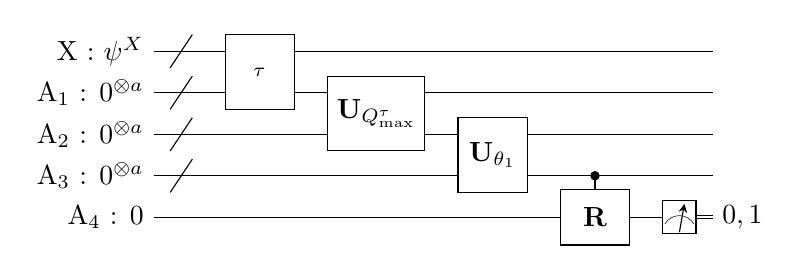
\begin{tikzpicture}[scale=1.000000,x=1pt,y=1pt]
\filldraw[color=white] (0.000000, -7.500000) rectangle (202.000000, 67.500000);
% Drawing wires
% Line 3: inputstate W \Ket{\psi}^X
\draw[color=black] (0.000000,60.000000) -- (202.000000,60.000000);
\draw[color=black] (0.000000,60.000000) node[left] {X : $\Ket{\psi}^X$};
% Line 4: qtau W \Ket{0}^{\otimes a}
\draw[color=black] (0.000000,45.000000) -- (202.000000,45.000000);
\draw[color=black] (0.000000,45.000000) node[left] {A$_1$ : $\Ket{0}^{\otimes a}$};
% Line 5: qtaunormalized W \Ket{0}^{\otimes a}
\draw[color=black] (0.000000,30.000000) -- (202.000000,30.000000);
\draw[color=black] (0.000000,30.000000) node[left] {A$_2$ : $\Ket{0}^{\otimes a}$};
% Line 6: theta W \Ket{0}^{\otimes a}
\draw[color=black] (0.000000,15.000000) -- (202.000000,15.000000);
\draw[color=black] (0.000000,15.000000) node[left] {A$_3$ : $\Ket{0}^{\otimes a}$};
% Line 7: cos W \Ket{0} {0,1}
\draw[color=black] (0.000000,0.000000) -- (190.000000,0.000000);
\draw[color=black] (190.000000,-0.500000) -- (202.000000,-0.500000);
\draw[color=black] (190.000000,0.500000) -- (202.000000,0.500000);
\draw[color=black] (0.000000,0.000000) node[left] {A$_4$ :   $\Ket{0}$};
% Done with wires; drawing gates
% Line 9: inputstate qtau qtaunormalized theta /
\draw (6.000000, 54.000000) -- (14.000000, 66.000000);
\draw (6.000000, 39.000000) -- (14.000000, 51.000000);
\draw (6.000000, 24.000000) -- (14.000000, 36.000000);
\draw (6.000000, 9.000000) -- (14.000000, 21.000000);
% Line 11: qtau inputstate G $\Or_\tau$ width=25 height=20
\draw (38.500000,60.000000) -- (38.500000,45.000000);
\begin{scope}
\draw[fill=white] (38.500000, 52.500000) +(-45.000000:17.677670pt and 19.091883pt) -- +(45.000000:17.677670pt and 19.091883pt) -- +(135.000000:17.677670pt and 19.091883pt) -- +(225.000000:17.677670pt and 19.091883pt) -- cycle;
\clip (38.500000, 52.500000) +(-45.000000:17.677670pt and 19.091883pt) -- +(45.000000:17.677670pt and 19.091883pt) -- +(135.000000:17.677670pt and 19.091883pt) -- +(225.000000:17.677670pt and 19.091883pt) -- cycle;
\draw (38.500000, 52.500000) node {$\Or_\tau$};
\end{scope}
% Line 12: qtaunormalized qtau G $\mathbf{U}_{Q_{\max}^{\tau}}$ width=35 height=20
\draw (80.500000,45.000000) -- (80.500000,30.000000);
\begin{scope}
\draw[fill=white] (80.500000, 37.500000) +(-45.000000:24.748737pt and 19.091883pt) -- +(45.000000:24.748737pt and 19.091883pt) -- +(135.000000:24.748737pt and 19.091883pt) -- +(225.000000:24.748737pt and 19.091883pt) -- cycle;
\clip (80.500000, 37.500000) +(-45.000000:24.748737pt and 19.091883pt) -- +(45.000000:24.748737pt and 19.091883pt) -- +(135.000000:24.748737pt and 19.091883pt) -- +(225.000000:24.748737pt and 19.091883pt) -- cycle;
\draw (80.500000, 37.500000) node {$\mathbf{U}_{Q_{\max}^{\tau}}$};
\end{scope}
% Line 13: theta qtaunormalized G $\mathbf{U}_{\theta_1}$ width=25 height=20
\draw (122.500000,30.000000) -- (122.500000,15.000000);
\begin{scope}
\draw[fill=white] (122.500000, 22.500000) +(-45.000000:17.677670pt and 19.091883pt) -- +(45.000000:17.677670pt and 19.091883pt) -- +(135.000000:17.677670pt and 19.091883pt) -- +(225.000000:17.677670pt and 19.091883pt) -- cycle;
\clip (122.500000, 22.500000) +(-45.000000:17.677670pt and 19.091883pt) -- +(45.000000:17.677670pt and 19.091883pt) -- +(135.000000:17.677670pt and 19.091883pt) -- +(225.000000:17.677670pt and 19.091883pt) -- cycle;
\draw (122.500000, 22.500000) node {$\mathbf{U}_{\theta_1}$};
\end{scope}
% Line 14: cos G $\mathbf{R}$ theta width=25 height=20
\draw (159.500000,15.000000) -- (159.500000,0.000000);
\begin{scope}
\draw[fill=white] (159.500000, -0.000000) +(-45.000000:17.677670pt and 14.142136pt) -- +(45.000000:17.677670pt and 14.142136pt) -- +(135.000000:17.677670pt and 14.142136pt) -- +(225.000000:17.677670pt and 14.142136pt) -- cycle;
\clip (159.500000, -0.000000) +(-45.000000:17.677670pt and 14.142136pt) -- +(45.000000:17.677670pt and 14.142136pt) -- +(135.000000:17.677670pt and 14.142136pt) -- +(225.000000:17.677670pt and 14.142136pt) -- cycle;
\draw (159.500000, -0.000000) node {$\mathbf{R}$};
\end{scope}
\filldraw (159.500000, 15.000000) circle(1.500000pt);
% Line 15: cos M
\draw[fill=white] (184.000000, -6.000000) rectangle (196.000000, 6.000000);
\draw[very thin] (190.000000, 0.600000) arc (90:150:6.000000pt);
\draw[very thin] (190.000000, 0.600000) arc (90:30:6.000000pt);
\draw[->,>=stealth] (190.000000, -5.400000) -- +(80:10.392305pt);
% Done with gates; drawing ending labels
\draw[color=black] (202.000000,0.000000) node[right] {${0,1}$};
% Done with ending labels; drawing cut lines and comments
% Done with comments
\end{tikzpicture}

  % \captionsetup{width=0.95\linewidth}
  \setcapwidth{0.95\linewidth}
  \caption{A quantum circuit representing a unitary operator $\U$ that achieves~\cref{eq:povm_implementation} for $\Lam=\sqrt{\uQ^{\tau}}$, which can be used for implementing a block encoding of $\sqrt{\uQ^{\tau}}$. This circuit achieves the transformations shown in \cref{eq:0}. The last controlled gate represents $\mathrm{C}\mathbf{R}$. Here, the system register $X$ consists of $D\lceil\log G\rceil$ qubits, and ancillary registers A$_{1-3}$ consist of $a=\O(\polylog\nicefrac{1}{\delta})$ qubits each.}
  \label{fig:q_tau}
  \end{figure}
%%%%%%%%%%%%%%%%%%%%%%%%%%%%%%%%%%%%%%%%%%%%%%%%%%%%%%%%%%%%



\begin{proof}
  First we construct a quantum circuit $\U$ that achieves~\cref{eq:povm_implementation} for $\Lam=\sqrt{\uQ^{\tau}}$.
  Denote an arbitrary input system state by
  \begin{equation}
    \Ket{\psi}^X=\sum_{\tv\in\tsX}\alpha_{\tv}\Ket{\tv}^X\in\sH^X.
  \end{equation}
  Define a function
  \begin{equation}
    \theta_1\left(q\right):=\arccos\left({q}^{\frac{1}{4}}\right).
  \end{equation}
  Let $\Rot_\theta$ denote the single qubit rotation $\ee^{-\ii\theta\sigma_y}$
  \begin{equation}
    \label{eq:rotation}
    \Rot_\theta:=\left(\begin{matrix}\cos\theta & -\sin\theta \\
    \sin\theta & \cos\theta\end{matrix}\right),
  \end{equation}
  and let $\mathrm{C}\Rot$ be the controlled rotation
  \begin{equation}
    \label{eq:controlled_rotation_q_tau}
    \mathrm{C}\Rot=\sum_{\theta}\ketbra{\theta}\otimes \Rot_\theta.
  \end{equation}
  Also assume we have circuits for unitary operators $\U_{Q_{\max}^{\tau}}$ and $\U_{\theta_1}$ % $\U_{G}$
  \begin{align}
    % \U_{G}\Ket{x}\Ket{0} &= \Ket{\frac{x}{G}}\nonumber\\
    \U_{Q_{\max}^{\tau}}\Ket{q}\Ket{0} &= \Ket{q}\Ket{\frac{q}{Q_{\max}^{\tau}}}\nonumber\\
    \U_{\theta_1}\Ket{q}\Ket{0} &= \Ket{q}\Ket{\theta_1(q)}.
  \end{align}
  The circuit of \cref{fig:q_tau} then achieves the following transformation (to precision $\delta$). First load the periodi  sed data density $Q$ of \cref{eq:Q-tau} % \label{eq:1}
  % \xrightarrow{  \U_{G}  }&\sum_{\tv}\alpha_{\tv}\Ket{\tv}\Ket{0}\Ket{0}\Ket{0}\Ket{0}\\
  \begin{align}
    \label{eq:0}
    \Ket{\psi}\Ket{0}\Ket{0}\Ket{0}\Ket{0}\quad
          \xrightarrow{  \Or_\tau  }\quad\sum_{\tv}\alpha_{\tv}\Ket{\tv}\Ket{Q^{\tau}\left(\tv\right)}\Ket{0}\Ket{0}\Ket{0},
  \end{align}
  then normalise by the maximum of $Q$, doing some quantum artihmetics,
  \begin{align}
    \label{eq:2}
    \ldots\xrightarrow{ \U_{Q_{\max}^{\tau}} }\quad\sum_{\tv}\alpha_{\tv}\Ket{\tv}\Ket{Q^{\tau}\left(\tv\right)}\Ket{\frac{Q^{\tau}\left(\tv\right)}{Q_{\max}^{\tau}}}\Ket{0}\Ket{0},
  \end{align}
  and then doing some inverse trigonometry,
  \begin{align}
    \label{eq:3}
    \ldots\xrightarrow{ \U_{\theta_1} }\quad\sum_{\tv}\alpha_{\tv}\Ket{\tv}\Ket{Q^{\tau}\left(\tv\right)}\Ket{\frac{Q^{\tau}\left(\tv\right)}{Q_{\max}^{\tau}}}\Ket{\theta_1\left(\frac{Q^{\tau}\left(\tv\right)}{Q_{\max}^{\tau}}\right)}\Ket{0}
  \end{align}
  and finally using the angle obtained to perform controlled rotations, we obtain
  \begin{align}
    \label{eq:4}
    \ldots\xrightarrow{ \mathrm{C}\Rot }\quad&\quad\sum_{\tv}\alpha_{\tv}\Ket{\tv}\Ket{Q^{\tau}\left(\tv\right)}\Ket{\frac{Q^{\tau}\left(\tv\right)}{Q_{\max}^{\tau}}}\Ket{\theta_1\left(\frac{Q^{\tau}\left(\tv\right)}{Q_{\max}^{\tau}}\right)}\nonumber\\
                                    &\quad\quad\left({\left(\frac{1}{Q_{\max}^{\tau}}Q^{\tau}\left(\tv\right)\right)}^{\frac{1}{4}}\Ket{0}+\sqrt{1-\sqrt{\frac{1}{Q_{\max}^{\tau}}Q^{\tau}\left(\tv\right)}}\Ket{1}\right).
  \end{align}
    % In~\cref{eq:1}, each of the $D$ elements of the vector $\tv$ in the first quantum register is multiplied by $\frac{1}{G}$ using arithmetics, and the result is stored in the second quantum register.
  % Since $\frac{1}{G}$ can be approximately represented with precision $O(\Delta)$ using $\O\left(\log\left(\frac{1}{\Delta}\right)\right)$ bits, these $D$ multiplications take $\O\left(D\log G \log\log G \polylog\frac{1}{\delta'}\right)$ time
  % due to~\cref{eq:runtime_multiplication}, which is dominant. % CAN THIS REALLY BE WHERE ALL THE D COMES FROM???
  The runtime of the quantum oracle $\Or_\tau$ queried in~\cref{eq:0} is $\O(1)$ modulo preprocessing cost for the QRAM; let us call it $T_\tau$. The quantum arithmetics for normalising by $Q_{\max}^{\tau}$ in~\cref{eq:2}, and calculating the inverse trigonometric function $\theta_1$ in~\cref{eq:3} incurs a circuit of size $a=\O\left(\polylog\nicefrac{1}{\delta'}\right)$ for a suitable precision $\delta'$~\cite{haner2018}.
  In~\cref{eq:4}, we rotate the single qubit register A$_4$ controlled on the angle computed and stored in A$_3$,
  needing $\O\left(a\right)$ gates since A$_3$ stores $\theta$ to $a$-bits of precision.
  Measuring the A$_4$ register, we get outcome $0$ with probability
  \begin{equation}
    \label{eq:probability_sqrt_q_tau}
    \Pr(\text{A}_4=0)=\sum_{\tv\in\tsX}{\left|\alpha_{\tv}\right|}^2 \sqrt{\frac{1}{Q_{\max}^{\tau}}Q^{\tau}\left(\tv\right)}=\tr\left[\Pi_{\psi}\sqrt{\uQ^{\tau}}\right],
  \end{equation}
  which achieves~\cref{eq:povm_implementation} for $\Lam=\sqrt{\uQ^{\tau}}$ within the claimed runtime.
\end{proof}

With the block-encoded $\sqrt{\uQ^{\tau}}$ as a building block, we next construct a block encoding of $\hSgOp_\epsilon$.
Note that while the following proposition provides a 
$$\left(1,\O\left(D\log G \polylog\frac{1}{\delta}\right),\delta\right)$$
 block encoding of $\left(1+\epsilon/Q_{\max}^{\tau}\right)^{-1}\hSgOp_\epsilon$, it is equivalently a 
$$\left(1+\epsilon/Q_{\max}^{\tau},\O\left(D\log G \polylog\frac{1}{\delta}\right),\left(1+\epsilon/Q_{\max}^{\tau}\right)\delta\right)$$
 block encoding of $\hSgOp_\epsilon$ by definition.
\begin{lemma}[Block encoding of $\hSgOp_\epsilon$]
  \label{sprp:block_encoding_sigma_lambda}
  For any $\epsilon>0$
  and any operator $\hSgOp_\epsilon$ of the form in \cref{eq:sigma-epsilon-full-rank},
  we can implement a $\left(1,s,\delta\right)$-block encoding of
  \begin{equation*}
    \frac{1}{1+\epsilon/Q_{\max}^{\tau}}\hSgOp_\epsilon
  \end{equation*}
  using a single query each to the quantum oracles $\Or_\rho^\dag$ and $\Or_\tau$, and $\O\left(s\log\log G\right)$ additional one- and two-qubit gates, with an ancillary register is of size
  \[s=\O\left(D\cdot\log G\cdot \poly\log\frac{1}{\delta}\right)\]
\end{lemma}

% \begin{figure}[t]
%   \centering
%   \includegraphics[width=6.5in]{sigma_lambda.pdf}
%   \caption{}
% \end{figure}
%%%%%%%%%%%%%%%%%%%%%%%%%%%%%%%%%%%%%%%%%%%%%%%%%%%%%%%%%%%%
\begin{figure}[!ht]
  \centering
  %! \usepackage{amsmath, amssymb, mathtools, braket}
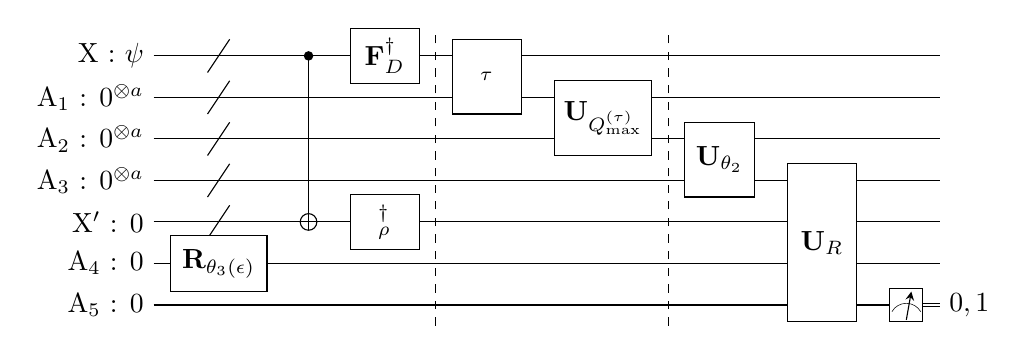
\begin{tikzpicture}[scale=1.000000,x=1pt,y=1pt]
\filldraw[color=white] (0.000000, -7.500000) rectangle (284.000000, 97.500000);
% Drawing wires
% Line 3: inputstate W \Ket{\psi}^X
\draw[color=black] (0.000000,90.000000) -- (284.000000,90.000000);
\draw[color=black] (0.000000,90.000000) node[left] {X : $\Ket{\psi}$};
% Line 4: qtau W \Ket{0}^{\otimes a}
\draw[color=black] (0.000000,75.000000) -- (284.000000,75.000000);
\draw[color=black] (0.000000,75.000000) node[left] {A$_1$ : $\Ket{0}^{\otimes a}$};
% Line 5: qtaunormalized W \Ket{0}^{\otimes a}
\draw[color=black] (0.000000,60.000000) -- (284.000000,60.000000);
\draw[color=black] (0.000000,60.000000) node[left] {A$_2$ : $\Ket{0}^{\otimes a}$};
% Line 6: theta W \Ket{0}^{\otimes a}
\draw[color=black] (0.000000,45.000000) -- (284.000000,45.000000);
\draw[color=black] (0.000000,45.000000) node[left] {A$_3$ : $\Ket{0}^{\otimes a}$};
% Line 7: aux W \Ket{0}^{X^\prime}
\draw[color=black] (0.000000,30.000000) -- (284.000000,30.000000);
\draw[color=black] (0.000000,30.000000) node[left] {X$'$ : $\Ket{0}$};
% Line 8: lambda W \Ket{0}
\draw[color=black] (0.000000,15.000000) -- (284.000000,15.000000);
\draw[color=black] (0.000000,15.000000) node[left] {A$_4$ : $\Ket{0}$};
% Line 9: cos W \Ket{0} {0,1}
\draw[color=black] (0.000000,0.000000) -- (272.000000,0.000000);
\draw[color=black] (272.000000,-0.500000) -- (284.000000,-0.500000);
\draw[color=black] (272.000000,0.500000) -- (284.000000,0.500000);
\draw[color=black] (0.000000,0.000000) node[left] {A$_5$ : $\Ket{0}$};
% Done with wires; drawing gates
% Line 11: inputstate qtau qtaunormalized theta aux /
\draw (19.500000, 84.000000) -- (27.500000, 96.000000);
\draw (19.500000, 69.000000) -- (27.500000, 81.000000);
\draw (19.500000, 54.000000) -- (27.500000, 66.000000);
\draw (19.500000, 39.000000) -- (27.500000, 51.000000);
\draw (19.500000, 24.000000) -- (27.500000, 36.000000);
% Line 16: lambda G $\mathbf{R}_{\theta_3\left(\epsilon\right)}$ width=35 height=20
\begin{scope}
\draw[fill=white] (23.500000, 15.000000) +(-45.000000:24.748737pt and 14.142136pt) -- +(45.000000:24.748737pt and 14.142136pt) -- +(135.000000:24.748737pt and 14.142136pt) -- +(225.000000:24.748737pt and 14.142136pt) -- cycle;
\clip (23.500000, 15.000000) +(-45.000000:24.748737pt and 14.142136pt) -- +(45.000000:24.748737pt and 14.142136pt) -- +(135.000000:24.748737pt and 14.142136pt) -- +(225.000000:24.748737pt and 14.142136pt) -- cycle;
\draw (23.500000, 15.000000) node {$\mathbf{R}_{\theta_3\left(\epsilon\right)}$};
\end{scope}
% Line 13: aux C inputstate
\draw (56.000000,90.000000) -- (56.000000,30.000000);
\begin{scope}
\draw[fill=white] (56.000000, 30.000000) circle(3.000000pt);
\clip (56.000000, 30.000000) circle(3.000000pt);
\draw (53.000000, 30.000000) -- (59.000000, 30.000000);
\draw (56.000000, 27.000000) -- (56.000000, 33.000000);
\end{scope}
\filldraw (56.000000, 90.000000) circle(1.500000pt);
% Line 14: aux G $\mathcal{O}_\rho^\dag$ width=25 height=20
\begin{scope}
\draw[fill=white] (83.500000, 30.000000) +(-45.000000:17.677670pt and 14.142136pt) -- +(45.000000:17.677670pt and 14.142136pt) -- +(135.000000:17.677670pt and 14.142136pt) -- +(225.000000:17.677670pt and 14.142136pt) -- cycle;
\clip (83.500000, 30.000000) +(-45.000000:17.677670pt and 14.142136pt) -- +(45.000000:17.677670pt and 14.142136pt) -- +(135.000000:17.677670pt and 14.142136pt) -- +(225.000000:17.677670pt and 14.142136pt) -- cycle;
\draw (83.500000, 30.000000) node {$\Or_\rho^\dag$};
\end{scope}
% Line 15: inputstate G $\mathbf{F}_D^\dag$ width=25 height=20
\begin{scope}
\draw[fill=white] (83.500000, 90.000000) +(-45.000000:17.677670pt and 14.142136pt) -- +(45.000000:17.677670pt and 14.142136pt) -- +(135.000000:17.677670pt and 14.142136pt) -- +(225.000000:17.677670pt and 14.142136pt) -- cycle;
\clip (83.500000, 90.000000) +(-45.000000:17.677670pt and 14.142136pt) -- +(45.000000:17.677670pt and 14.142136pt) -- +(135.000000:17.677670pt and 14.142136pt) -- +(225.000000:17.677670pt and 14.142136pt) -- cycle;
\draw (83.500000, 90.000000) node {$\mathbf{F}_D^\dag$};
\end{scope}
% Line 17: inputstate qtau qtaunormalized theta aux lambda cos TOUCH style=dashed
\draw[dashed] (102.000000,-7.500000) -- (102.000000,97.500000);
% Line 18: qtau inputstate G $\mathcal{O}_\tau$ width=25 height=20
\draw (120.500000,90.000000) -- (120.500000,75.000000);
\begin{scope}
\draw[fill=white] (120.500000, 82.500000) +(-45.000000:17.677670pt and 19.091883pt) -- +(45.000000:17.677670pt and 19.091883pt) -- +(135.000000:17.677670pt and 19.091883pt) -- +(225.000000:17.677670pt and 19.091883pt) -- cycle;
\clip (120.500000, 82.500000) +(-45.000000:17.677670pt and 19.091883pt) -- +(45.000000:17.677670pt and 19.091883pt) -- +(135.000000:17.677670pt and 19.091883pt) -- +(225.000000:17.677670pt and 19.091883pt) -- cycle;
\draw (120.500000, 82.500000) node {$\Or_\tau$};
\end{scope}
% Line 19: qtaunormalized qtau G $\mathbf{U}_{Q_{\max}^{\left(\tau\right)}}$ width=35 height=20
\draw (162.500000,75.000000) -- (162.500000,60.000000);
\begin{scope}
\draw[fill=white] (162.500000, 67.500000) +(-45.000000:24.748737pt and 19.091883pt) -- +(45.000000:24.748737pt and 19.091883pt) -- +(135.000000:24.748737pt and 19.091883pt) -- +(225.000000:24.748737pt and 19.091883pt) -- cycle;
\clip (162.500000, 67.500000) +(-45.000000:24.748737pt and 19.091883pt) -- +(45.000000:24.748737pt and 19.091883pt) -- +(135.000000:24.748737pt and 19.091883pt) -- +(225.000000:24.748737pt and 19.091883pt) -- cycle;
\draw (162.500000, 67.500000) node {$\mathbf{U}_{Q_{\max}^{\left(\tau\right)}}$};
\end{scope}
% Line 20: inputstate qtau qtaunormalized theta aux lambda cos TOUCH style=dashed
\draw[dashed] (186.000000,-7.500000) -- (186.000000,97.500000);
% Line 21: theta qtaunormalized G $\mathbf{U}_{\theta_2}$ width=25 height=20
\draw (204.500000,60.000000) -- (204.500000,45.000000);
\begin{scope}
\draw[fill=white] (204.500000, 52.500000) +(-45.000000:17.677670pt and 19.091883pt) -- +(45.000000:17.677670pt and 19.091883pt) -- +(135.000000:17.677670pt and 19.091883pt) -- +(225.000000:17.677670pt and 19.091883pt) -- cycle;
\clip (204.500000, 52.500000) +(-45.000000:17.677670pt and 19.091883pt) -- +(45.000000:17.677670pt and 19.091883pt) -- +(135.000000:17.677670pt and 19.091883pt) -- +(225.000000:17.677670pt and 19.091883pt) -- cycle;
\draw (204.500000, 52.500000) node {$\mathbf{U}_{\theta_2}$};
\end{scope}
% Line 22: cos theta aux lambda G $\mathbf{U}_R$ width=25 height=20
\draw (241.500000,45.000000) -- (241.500000,0.000000);
\begin{scope}
\draw[fill=white] (241.500000, 22.500000) +(-45.000000:17.677670pt and 40.305087pt) -- +(45.000000:17.677670pt and 40.305087pt) -- +(135.000000:17.677670pt and 40.305087pt) -- +(225.000000:17.677670pt and 40.305087pt) -- cycle;
\clip (241.500000, 22.500000) +(-45.000000:17.677670pt and 40.305087pt) -- +(45.000000:17.677670pt and 40.305087pt) -- +(135.000000:17.677670pt and 40.305087pt) -- +(225.000000:17.677670pt and 40.305087pt) -- cycle;
\draw (241.500000, 22.500000) node {$\mathbf{U}_R$};
\end{scope}
% Line 23: cos M
\draw[fill=white] (266.000000, -6.000000) rectangle (278.000000, 6.000000);
\draw[very thin] (272.000000, 0.600000) arc (90:150:6.000000pt);
\draw[very thin] (272.000000, 0.600000) arc (90:30:6.000000pt);
\draw[->,>=stealth] (272.000000, -5.400000) -- +(80:10.392305pt);
% Done with gates; drawing ending labels
\draw[color=black] (284.000000,0.000000) node[right] {${0,1}$};
% Done with ending labels; drawing cut lines and comments
% Done with comments
\end{tikzpicture}

  % \captionsetup{width=0.95\linewidth}
  \setcapwidth{0.95\linewidth}
  \caption{Quantum circuit for $\U$ that achieves~\cref{eq:povm_implementation} for $\Lam=\hSgOp_\epsilon$, which can be used for implementing a block encoding of $\hSgOp_\epsilon$. The first controlled-not collectively represents $\CNOT$ gates on corresponding pairs of qubits of $X$ and $X'$. % The part of this circuit between the vertical dashed lines also occurs in \cref{fig:q_tau}.
  % Additionally, the circuit performs a preprocessing of the input state before performing the part corresponding to \cref{fig:q_tau},
  This circuit achieves the series of transformations starting from~\cref{eq:state_transformation}. Measuring register A$_5$ produces outcomes in accordance with \cref{eq:probability}.
  % The last two unitaries $\U_{\theta_2}$ and $\U_R$ after the part corresponding to \cref{fig:q_tau}, which are followed by a measurement described by the analysis starting from~\cref{eq:probability}. 
  Here, $a=\O(\polylog\nicefrac{1}{\epsilon})$.}
  \label{fig:sigma_lambda}
\end{figure}
%%%%%%%%%%%%%%%%%%%%%%%%%%%%%%%%%%%%%%%%%%%%%%%%%%%%%%%%%%%%


\begin{proof}
  We will first construct a circuit $\U$ that achieves~\cref{eq:povm_implementation} for $\Lam=\hSgOp_\epsilon$, using the same notation as in \cref{sprp:block_encoding_q_tau}. Let
  \begin{equation}
    \label{eq:psi}
    \Ket{\psi}^X=\sum_{\tx\in\tsX}\alpha_{\tx}\Ket{\tx}^X\in\sH^X.
  \end{equation}
  be an arbitrary input system state, and define functions
  \begin{align}
    \theta_2\left(q\right)&:=\arccos\left(\sqrt{q}\right),\\
    \theta_3\left(\epsilon\right)&:=\arccos\left(\sqrt{\frac{\epsilon/Q_{\max}^{\tau}}{1+\epsilon/Q_{\max}^{\tau}}}\right).
  \end{align}
  Since these are efficiently computable elementary functions, we again have efficient circuits for the quantum arithmetics, for instance
  \begin{align}
    \label{eq:U_theta_2}
    \U_{\theta_2}\Ket{q}\Ket{0} = \Ket{q}\Ket{\theta_2(q)}.
  \end{align}
  % Let $\Or_\rho$ denote a unitary operator representing a quantum circuit for implementing the oracle $\Or_\rho$.
  % Then, the unitary operator representing its inverse $\Or_\rho^\dag$ is given by $\Or_\rho^\dag$.
  We will also need the multi-controlled rotation (as before, $\Pi_\theta:=\ketbra{\theta}$ etc.\ are projectors)
  \begin{align}
    \label{eq:controlled_rotation_sigma_lambda}
    \U_R=&\left(\id^{\text{A}_3}\otimes\id^{X'}\otimes\Pi_0^{\text{A}_4}\otimes\id^{\text{A}_5}\right)   +  
        \left(\sum_{\theta}\Pi_{\theta}^{\text{A}_3}\otimes\left(\id-\Pi_0\right)^{X'}\otimes\Pi_{1}^{\text{A}_4}\otimes \sigma_x^{\text{A}_5}\right)\nonumber\\
        &\qquad+\left(\sum_{\theta}\Pi_{\theta}^{\text{A}_3}\otimes\Pi_0^{X'}\otimes\Pi_{1}^{\text{A}_4}\otimes \Rot_\theta^{\text{A}_5}\right).
  \end{align}

  Let us now analyse the quantum circuit of \cref{fig:sigma_lambda}, with these ingredients in place.
  The part of this circuit in between the vertical dashed lines also appears in \cref{fig:q_tau}. The preprocessing before the first vertical line effects the transformation
  \begin{align}
    \label{eq:state_transformation}
    &\Ket{\psi}^X\Ket{0}\Ket{0}\Ket{0}\Ket{0}^{X'}\Ket{0}^{\text{A}_4}\Ket{0}^{\text{A}_5}\\
    \label{eq:cnot_used}
    \xrightarrow{\CNOT}&\sum_{\tx}\alpha_{\tx}\Ket{\tx}^X\Ket{0}\Ket{0}\Ket{0}\Ket{\tx}^{X'}\Ket{0}^{\text{A}_4}\Ket{0}^{\text{A}_5}\\
    \label{eq:f_d_used}
    \xrightarrow{\F_{D}^\dag\otimes\Or_\rho^\dag\otimes \Rot_{\theta_3\left(\epsilon\right)}}&\sum_{\tx}\alpha_{\tx}\F_{D}^\dag\Ket{\tx}^X\Ket{0}\Ket{0}\Ket{0} \Or_\rho^\dag\Ket{\tx}^{X'}\nonumber\\
                    &\quad\left(\sqrt{\frac{\epsilon/Q_{\max}^{\tau}}{1+\epsilon/Q_{\max}^{\tau}}}\Ket{0}^{\text{A}_4}+\sqrt{\frac{1}{1+\epsilon/Q_{\max}^{\tau}}}\Ket{1}^{\text{A}_4}\right)\otimes\Ket{0}^{\text{A}_5}.
  \end{align}
  In~\cref{eq:cnot_used}, $\CNOT$ gates on each of the $\O\left(D\log G \right)$ qubits of the quantum registers $X$ and $X'$ copy out the basis states into the register $X'$.
  $\F_{D}^\dag$ in~\cref{eq:f_d_used} requires $\widetilde{\O}\left(D\log G\right)$ gates as we saw in~\cref{eq:runtime_F_D}. $\Or_\rho^\dag$ queries QRAM and so it costs only $\O(1)$ in lookup (addressing) time, but say the preprocessing (state preparation) time is $T_\rho$. The single qubit rotation $\Rot_{\theta_3\left(\epsilon\right)}$ of \cref{eq:rotation} can be implemented with precision $O(\delta')$ using $\O\left(\polylog\frac{1}{\delta'}\right)$ gates~\cite{Nielsen2010}.

  Next comes the part that was also in \cref{fig:q_tau}. Following this, we implement $\U_{\theta_2}$ as we did in \cref{eq:3}, using $\O\left(\polylog\frac{1}{\delta'}\right)$ gates.
  We can implement $\U_R$ using $\O\left(D\log G \polylog\frac{1}{\delta'}\right)$ gates since $\Ket{\theta}$ is stored in $\O\left(\polylog\frac{1}{\delta'}\right)$ qubits and $X'$ consists of $\O\left(D\log G \right)$ qubits.

  After performing $\U_R$, we measure the last qubit A$_5$ in the computational basis. We will calculate the probability of obtaining the outcome $0$ in this measurement of A$_5$ using conditional probabilities; suppose that we performed a measurement of the one-qubit register A$_4$ in the computational basis. The outcome probabilities are
  \begin{align}
    \label{eq:ancilla_a4_probs}
    \Pr(\text{A}_4=0) &= \frac{\epsilon/Q_{\max}^{\tau}}{1+\epsilon/Q_{\max}^{\tau}}\nonumber\\
    \Pr(\text{A}_4=1) &= \frac{1}{1+\epsilon/Q_{\max}^{\tau}}.
  \end{align} 
  Conditioned on seeing $\text{A}_4=0$, measuring A$_5$ gives outcome $0$ with certainty, corresponding to the first term of~\cref{eq:controlled_rotation_sigma_lambda}.
  Similarly, the third term of~\cref{eq:controlled_rotation_sigma_lambda} tells us that
  \begin{align}
    \label{eq:probability}
    \Pr(\text{A}_5=0~|~\text{A}_4=1)&=\sum_{\tx'\in\tsX}{\left|\sum_{\tx\in\tsX}\alpha_{\tx}\Braket{\tx'|\F_{D}^\dag|\tx}\Braket{0|\Or_\rho^\dag|\tx}\sqrt{\frac{1}{Q_{\max}^{\tau}}Q^{\tau}\left(\frac{\tx'}{G}\right)}\right|}^2\nonumber\\
    &=\sum_{\tx'\in\tsX}\frac{1}{Q_{\max}^{\tau}}Q^{\tau}\left(\frac{\tx'}{G}\right){\left|\sum_{\tx\in\tsX}\alpha_{\tx}\Braket{\tx'|\F_{D}^\dag|\tx}\Braket{0|\Or_\rho^\dag|\tx}\right|}^2.
  \end{align}
  The second term of~\cref{eq:controlled_rotation_sigma_lambda} makes no contribution to~\cref{eq:probability} because $\sigma_x$ flips $\Ket{0}$ to $\Ket{1}$. 
  Recall that by definition of $\Or_\rho$,
  \begin{equation*}
  \tag{I'm \ref{eq:oracle_rho_definition}}
  \Or_\rho\Ket{0}=\sum_{\tx\in\tsX}\sqrt{\hq^{\rho}(\tx)}\Ket{\tx}
  =\sqrt{\hbq^{\rho}}\sum_{\tx\in\tsX}\Ket{\tx}.
  \end{equation*}
  This means that  $${\left|\Braket{0|\Or_\rho^\dag|\tx}\right|}=\sqrt{\hq^{\rho}(\tx)}.$$ We then have  
  \begin{align}
    \label{eq:probability2}\cref{eq:probability}&=\sum_{\tx'\in\tsX}\frac{1}{Q_{\max}^{\tau}}Q^{\tau}\left(\frac{\tx'}{G}\right){\left|\sum_{\tx\in\tsX}\alpha_{\tx}\Braket{\tx'|\F_{D}^\dag|\tx}\sqrt{\hq^{\rho}(\tx)}\right|}^2\nonumber\\
    &=\sum_{\tx'\in\tsX}\frac{1}{Q_{\max}^{\tau}}Q^{\tau}\left(\frac{\tx'}{G}\right){\left|\sum_{\tx\in\tsX}\alpha_{\tx}\Braket{\tx'|\F_{D}^\dag\sqrt{\hbq^{\rho}}|\tx}\right|}^2.
  \end{align}
  By definition~\cref{eq:psi} of $\Ket{\psi}$, we have
  \begin{align}
    \label{eq:probability3}\cref{eq:probability2}&=\sum_{\tx'\in\tsX}\frac{1}{Q_{\max}^{\tau}}Q^{\tau}\left(\frac{\tx'}{G}\right){\left|\Braket{\tx'|\F_{D}^\dag\sqrt{\hbq^{\rho}}|\psi}\right|}^2\nonumber\\
    &=\sum_{\tx'\in\tsX}\frac{1}{Q_{\max}^{\tau}}Q^{\tau}\left(\frac{\tx'}{G}\right)\Braket{\tx'|\F_{D}^\dag\sqrt{\hbq^{\rho}}\Pi_{\psi}\sqrt{\hbq^{\rho}}\F_{D}|\tx'}\nonumber\\
    &=\frac{1}{Q_{\max}^{\tau}}\tr\left[\F_{D}^\dag\sqrt{\hbq^{\rho}}\Pi_{\psi}\sqrt{\hbq^{\rho}}\F_{D}\left(\sum_{\tx'\in\tsX}Q^{\tau}\left(\frac{\tx'}{G}\right)\Ket{\tx'}\Bra{\tx'}\right)\right].
  \end{align}
  By definition~\cref{eq:q_tau_g} of $\Q^{\tau}$, this is the same as
  \begin{align}
    \label{eq:probability4}\cref{eq:probability3}&=\frac{1}{Q_{\max}^{\tau}}\tr\left[\F_{D}^\dag\sqrt{\hbq^{\rho}}\Pi_{\psi}\sqrt{\hbq^{\rho}}\F_{D} \Q^{\tau}\right]\nonumber\\
    &=\frac{1}{Q_{\max}^{\tau}}\tr\left[\Pi_{\psi}\sqrt{\hbq^{\rho}}\F_{D} \Q^{\tau}\F_{D}^\dag\sqrt{\hbq^{\rho}}\right]\nonumber\\
    &=\frac{1}{Q_{\max}^{\tau}}\tr\left[\Pi_{\psi}\sqrt{\hbq^{\rho}}\krn\sqrt{\hbq^{\rho}}\right],
  \end{align}
  where the last equality follows from the perfect reconstruction of the kernel $k$ shown in \cref{prop:perfect_recon}.
  Therefore, plugging in the probabilities for measurements on A$_4$ from \cref{eq:ancilla_a4_probs}, we obtain
  \begin{align}
    \Pr(\text{A}_5=0)&=\frac{\epsilon/Q_{\max}^{\tau}}{1+\epsilon/Q_{\max}^{\tau}}\times 1+\frac{1}{1+\epsilon/Q_{\max}^{\tau}}\times\left(\frac{1}{Q_{\max}^{\tau}}\tr\left[\Pi_{\psi}\sqrt{\hbq^{\rho}}\krn\sqrt{\hbq^{\rho}}\right]\right)\nonumber\\
    &=\frac{1}{1+\epsilon/Q_{\max}^{\tau}}\times \tr\left[\Pi_{\psi}\left(\frac{\epsilon}{Q_{\max}^{\tau}}\id\right)\right]+\frac{1}{1+\epsilon/Q_{\max}^{\tau}}\times\tr\left[\Pi_{\psi}\left(\frac{1}{Q_{\max}^{\tau}}\sqrt{\hbq^{\rho}}\krn\sqrt{\hbq^{\rho}}\right)\right]\nonumber\\
    &=\frac{1}{1+\epsilon/Q_{\max}^{\tau}}\times \tr\left[\Pi_{\psi}\left(\frac{1}{Q_{\max}^{\tau}}\sqrt{\hbq^{\rho}}\krn\sqrt{\hbq^{\rho}}+\frac{\epsilon}{Q_{\max}^{\tau}}\id\right)\right]\nonumber\\
    &=\tr\left[\Pi_{\psi}\left(\frac{1}{1+\epsilon/Q_{\max}^{\tau}}\hSgOp_\epsilon\right)\right],
  \end{align}
  where the last equality follows from the definition~\cref{eq:sigma-epsilon-full-rank} of $\hSgOp_\epsilon$ (\cref{sec:featureSamp_state}).
  This achieves~\cref{eq:povm_implementation} for $\Lam=\frac{1}{1+\epsilon/Q_{\max}^{\tau}}\hSgOp_\epsilon$ within the claimed circuit size.
\end{proof}

We can now bound the runtime of \cref{alg:random_feature_revised} using the analyses for these block encodings in \cref{sprp:block_encoding_q_tau,sprp:block_encoding_sigma_lambda}.

\begin{proof}[Proof of \cref{thm:sampling}]
  The most resource intensive step of \cref{alg:random_feature_revised} is Step~5, as can be seen in the following.

  In Step~2, we prepare $\sum_{\tx}\Ket{0}^X\otimes\sqrt{\hbq^{\rho}}\Ket{\tx}^{X'}$ by one query to the oracle $\Or_\rho$, followed by $\O\left(D\log G \right)$ $\CNOT$ gates to prepare $\sum_{\tx}\Ket{\tx}^X\otimes\sqrt{\hbq^{\rho}}\Ket{\tx}^{X'}$, since $\sH^X$ consists of $\O\left(D\log G \right)$ qubits.
Step~3 performs $\F_{D}^\dag$, which is implemented using $\widetilde{\O}\left(D\log G\right)$ gates as shown in~\cref{eq:runtime_F_D}.
Step~4 is the block encoding of $\sqrt{\uQ^{\tau}}$, requiring $\widetilde{\O}\left(D\log G +T_\tau\right)$ gates as shown in \cref{sprp:block_encoding_q_tau}.
The runtime at this moment is $\widetilde{\O}\left(D\log G+T_\rho+T_\tau\right)$.
After Step-4, the part of the state we are interested in is
\begin{equation}
  \label{eq:state_to_amplify}
  \sum_{\tx\in\tsX}\Ket{\tx}^X\otimes \sqrt{\uQ^{\tau}}\F_{D}^\dag\sqrt{\hbq^{\rho}}\Ket{\tx}^{X'}.
\end{equation}
The norm of this term is
\begin{align}
  \left\|\sum_{\tx\in\tsX}\Ket{\tx}^X\otimes \sqrt{\uQ^{\tau}}\F_{D}^\dag\sqrt{\hbq^{\rho}}\Ket{\tx}^{X'}\right\|_2 &=\sqrt{\frac{\tr\left[\sqrt{\hbq^{\rho}} \F_{D} \Q^{\tau}\F_{D}^\dag\sqrt{\hbq^{\rho}}\right]}{Q_{\max}^{\tau}}}\nonumber\\
  &=\sqrt{\frac{\tr\left[\F_{D} \Q^{\tau}\F_{D}^\dag\hbq^{\rho}\right]}{Q_{\max}^{\tau}}}\nonumber\\
  &=\sqrt{\frac{\tr\hSgOp}{Q_{\max}^{\tau}}},
\end{align}
where the last equality uses $\hSgOp=\krn\hbq^{\rho}=\F_D \Q^{\tau} \F_D^\dag \hbq^{\rho}$ obtained from \cref{prop:perfect_recon}.
For any translation-invariant kernel $\tk(x',x)=\tk\left(x'-x\right)$, we can evaluate $\tr\hSgOp$ as
\begin{equation}
  \tr\hSgOp=\tr \left[\krn \hbq^{\rho}\right]=\tk(0)\tr \hbq^{\rho}=\tk(0,0)=\Omega(1),
\end{equation}
where we use the mild assumption $\tk(0,0)=\Omega(k(0,0))=\Omega(1)$ that we'd discussed in \cref{app:perfect_recon}.
Thus, to obtain the normalised quantum state proportional to the term~\cref{eq:state_to_amplify}, Step~4 is followed by standard amplitude amplification, repeating the above steps $$\O\left(\sqrt{\frac{Q_{\max}^{\tau}}{\tr\hSgOp}}\right)=\O\left(\sqrt{Q_{\max}^{\tau}}\right)$$ times.
Therefore, at the end of Step~4 including the amplitude amplification, the runtime is
\begin{equation}
  \label{eq:step_4}
  \O\left(\left(D\log G \log\log G \polylog\frac{1}{\delta}+T_\rho+T_\tau\right)\times\sqrt{Q_{\max}^{\tau}}\right).
\end{equation}
Step~5 performs a block encoding of $\hSgOp_\epsilon^{-\frac{1}{2}}$, which is obtained from quantum singular value transformation (QSVT) of the block encoding $\U_{\hSgOp}$ of $\left(1+\epsilon/Q_{\max}^{\tau}\right)^{-1}\hSgOp_\epsilon$ constructed in \cref{sprp:block_encoding_sigma_lambda}.
The QSVT combined with variable-time amplitude amplification~\cite{Ambainis2012VariableTimeAmpAmp,Chakraborty2018TheSimulation} yields a block encoding of ${\left(\frac{1}{1+(\epsilon/Q_{\max}^{\tau})}\hSgOp_\epsilon\right)}^{-\frac{1}{2}}$, using $\U_{\hSgOp}$ 
 $$\widetilde{O}\left({\left(\frac{Q_{\max}^{\tau}}{\epsilon}+1\right)}\polylog\frac{1}{\delta'}\right)$$ 
 times~\cite{Gilyen2018QuantumArithmetics}. This includes amplitude amplification,
and $\frac{Q_{\max}^{\tau}}{\epsilon}+1$ is the condition number of $\frac{1}{1+(\epsilon/Q_{\max}^{\tau})}\hSgOp_\epsilon$ since it holds that
\begin{equation}
  \frac{1}{1+(\epsilon/Q_{\max}^{\tau})}\frac{\epsilon}{Q_{\max}^{\tau}}\id\leq\frac{1}{1+(\epsilon/Q_{\max}^{\tau})}\hSgOp_\epsilon\leq\id.
\end{equation}
Thus, the net runtime/circuit size for Step~5  is
\begin{align}
  \label{eq:step_5}
  \O\left(D\log G \log\log G +T_\rho+T_\tau\right)\times\widetilde{O}\left(\frac{Q_{\max}^{\tau}}{\epsilon}\polylog\frac{1}{\delta}\right).
\end{align}
Finally, from~\cref{eq:step_4} and~\cref{eq:step_5}, the total runtime of quOptRF at the end of Step~5, including all amplitude amplification steps, is 
\begin{align}
  &\O\left(D\log G \log\log G +T_\rho+T_\tau\right)\times\widetilde{O}\left({\left(\sqrt{Q_{\max}^{\tau}}+\frac{Q_{\max}^{\tau}}{\epsilon}\right)}\polylog\frac{1}{\delta}\right)\nonumber\\
  &=\widetilde{\O}\left(D\log G\cdot\frac{Q_{\max}^{\tau}}{\epsilon}\cdot\polylog\frac{1}{\delta}\right),
\end{align}
establishing our claim.
\end{proof}

%%%%%%%%%%%%%%%%%%%%%%%%%%%%%%%%%%%%%%%%%%%%%%%%%%%%%%%%%
\setcounter{equation}{0}
\section{The runtime of SGD: Proof of \texorpdfstring{\cref{thm:overall_complexity}}{Theorem 4.4}}
\label{app:featureSamp_runtime}

Finally, we prove \cref{thm:overall_complexity} bounding the overall runtime of the supervised learning with optimised random features.
\cref{alg:sgd,alg:data_approximation} for stochastic gradient descent (SGD) and achieving the supervised learning respectively are also repeated in the following.

{
% \settheoremtag{\ref{thm:overall_complexity} again} % was Theorem*
\begin{theorem*}[Overall runtime of supervised learning by optimised random features]
  The runtime of \cref{alg:data_approximation} is
  \begin{equation*}
    O\left(MT\right)+O\left(\left(MD+T_{\tx}+T_y\right)\frac{1}{{\epsilon}^2 Q_{\min}^2}\log\frac{1}{\delta}\right),
  \end{equation*}
  where $T$ is the runtime of quOptRF, $M$ is the number of optimised random features to be sampled using by \cref{alg:random_feature_revised}, and the second term is runtime of the SGD\@.
  In particular, this is as fast as linear in $M$ and $D$, i.e.\
  $\O\left(MD\right)$.
\end{theorem*}
}

Recall that to perform the SGD, we invoke classical RAM oracles for accessing data
\begin{equation*}
  \tag{I'm \ref{eq:classical_oracles}}
 \Or_{\tx}(n)=\tx_n,\quad \Or_y(n)=y_n.
\end{equation*}

%%%%%%%%%%%%%%%%%%%%%%%%%%%%%%%%%%%%%%%%%%%%%%%%%%%%%%%%%%%
\begin{algorithm}[H]
  \setstretch{1.7}
  \caption*{\cref{alg:sgd} again: Descending stochastically using the gradient}
  \begin{algorithmic}[1]
    \Require{A function $I:\sW\to\R$, a projection $\Pi$ to a convex parameter region $\sW\subset\R^M$, a fixed number of iterations $T\in\mathbb{N}$, an initial point $\alpha^1\in\sW$, $T$-dependent hyperparameters representing step sizes $\left(\eta^{(t)}:t=1,\ldots,T\right)$ given in~\cite{pmlr-v99-jain19a}.}
    \Ensure{Approximate solution $\alpha$ minimising $I(\alpha)$.}
    \For{$t\in\left\{1,\ldots,T\right\}$}
    \State{Calculate $\hg^{(t)}$ satisfying $\mathbb{E}\left[\hg^{(t)}\right]=\nabla I(\alpha^{(t)})$.}
    \State{$\alpha^{\left(t+1\right)}\gets\Pi(\alpha^{(t)}-\eta^{(t)} \hg^{(t)})$.}
    \EndFor%
    \State{\textbf{Return } $\alpha\gets\alpha^{(T+1)}$.}
  \end{algorithmic}
\end{algorithm}
%%%%%%%%%%%%%%%%%%%%%%%%%%%%%%%%%%%%%%%%%%%%%%%%%%%%%%%%%%%
\begin{algorithm}[H]
  \setstretch{1.7}
  \caption*{\cref{alg:data_approximation} again: quOptRF for supervised learning.}
  \begin{algorithmic}[1]
    \Require{Inputs to \cref{alg:random_feature_revised,alg:sgd}, required number $M$ of features for achieving  the learning to accuracy $O({\epsilon})$, classical oracles $\Or_{\tx},\Or_y$ in~\cref{eq:classical_oracles}.}
    \Ensure{Optimised random features $v_0,\ldots,v_{M-1}$ and coefficients $\alpha_0,\ldots,\alpha_{M-1}$ for $\sum_m\alpha_m\varphi(v_m,\cdot)$ to achieve the learning with probability greater than $1-\delta$.}
    \For{$m\in\left\{0,\ldots,M-1\right\}$}
    \State{$v_m\gets\textrm{quOptRF}$.}~\Comment{by \cref{alg:random_feature_revised}.}
    \EndFor%
    \State{Minimise $I(\alpha)$ to accuracy $O({\epsilon})$ by \textrm{SGD} to obtain $\alpha_0,\ldots,\alpha_{M-1}$.}~\Comment{by \cref{alg:sgd}.}
    \State{\textbf{Return }$v_0,\ldots,v_{M-1},\alpha_0,\ldots,\alpha_{M-1}$.}
  \end{algorithmic}
\end{algorithm}
%%%%%%%%%%%%%%%%%%%%%%%%%%%%%%%%%%%%%%%%%%%%%%%%%%%%%%%%%%%

\begin{proof}
  Let us look at \cref{alg:data_approximation} step-by-step.
  In Step~2, using \cref{alg:random_feature_revised} repeatedly $M$ times, we can obtain $M$ optimised random features within time
  \begin{equation}
    \label{eq:algorithm_1}
    O(MT_q),
  \end{equation}
  where $T_q$ is the runtime of quOptRF as given by \cref{thm:sampling}.
  As for Step~4, we bound the runtime of the SGD in \cref{alg:sgd}.
  In the following, we show that the runtime of each iteration of the SGD is $\O\left(MD+T_{\tx}+T_y\right)$, and the required number of iterations in the SGD is upper bounded by $\O\left(\frac{1}{{\epsilon}^2 Q_{\min}^2}\log\frac{1}{\delta}\right)$.

  Consider the $t$\textsuperscript{th} iteration of the SGD for $t\in\left\{0,\ldots,T-1\right\}$.
  The most intensive step is the calculation of an unbiased estimate $\hg^{(t)}$ of the gradient $\mathbb{E}\left[\hg^{(t)}\right]=\nabla I\left(\alpha^{(t)}\right)$ for
  \begin{equation}
    I\left(\alpha\right):=\sum_{\tx\in\tsX}p^{\rho}(\tx){\left|f(\tx)-\sum_{m=0}^{M-1}\alpha_{m}\varphi\left(v_m,\tx\right)\right|}^2,
  \end{equation}
  where $\varphi(v,x)=\ee^{-2\pi\ii v\cdot x}$, $p^{\rho}(\tx)=\int_{\Delta_{\tx}}d\rho(x)$, and we write 
  \begin{equation}
    \alpha=\left(\begin{matrix}
        \alpha_{0}\\
        \vdots\\
        \alpha_{M-1}
    \end{matrix}\right).
  \end{equation}
The gradient of $I$ is given by
\begin{align}
  \label{eq:nabla_I}
  \nabla I\left(\alpha\right)&=
  \sum_{\tx\in\tsX}p^{\rho}(\tx)\left(\begin{matrix}2\Re\left[ \ee^{-2\pi\ii v_0\cdot \tx}\left(f(\tx)-\sum_{m=0}^{M-1}\alpha_m\ee^{2\pi\ii v_m\cdot \tx}\right)\right]\\
                 \vdots\\
                 2\Re\left[ \ee^{-2\pi\ii v_{M-1}\cdot \tx}\left(f(\tx)-\sum_{m=0}^{M-1}\alpha_m\ee^{2\pi\ii v_m\cdot \tx}\right)\right]
         \end{matrix}\right)\nonumber\\
                             &=\sum_{m=0}^{M-1}\frac{1}{M}\sum_{\tx\in\tsX}p^{\rho}(\tx)\left(\begin{matrix}2\Re\left[ \ee^{-2\pi\ii v_0\cdot \tx}\left(f(\tx)-M\alpha_m\ee^{2\pi\ii v_m\cdot \tx}\right)\right]\\
                 \vdots\\
                 2\Re\left[\ee^{-2\pi\ii v_{M-1}\cdot \tx}\left(f(\tx)-M\alpha_m\ee^{2\pi\ii v_m\cdot \tx}\right)\right]
         \end{matrix}\right),
\end{align}
where $\Re$ represents the real part.
In the $t$\textsuperscript{th} iteration, \cref{alg:sgd} estimates the gradient at the point $\alpha_{0}^{(t)}\in\left\{\alpha^{(1)},\ldots,\alpha^{(t)}\right\}$
% \begin{equation}
%   \alpha^{(t)}=\left(\begin{matrix}
%       \alpha_{0}^{(t)}\\
%       \vdots\\
%       \alpha_{M-1}^{(t)}
%   \end{matrix}\right)\in\left\{\alpha^1,\ldots,\alpha^{(t)}\right\}.
% \end{equation}

Using a pair of given data points $\left(\tx_t,y_t=f\left(\tx_t\right)\right)\in\left\{\left(\tx_{0},y_{0}\right),\left(\tx_{1},y_{1}\right),\ldots,\right\}$ sampled with probability $p^{\rho}(\tx)$ as observations of an independently and identically distributed (IID) random variable, and an integer $m\in\left\{0,\ldots,M-1\right\}$ uniformly sampled with probability $\frac{1}{M}$, we give an unbiased estimate $\hg^{(t)}$ of this gradient at each point $\alpha^{(t)}$ by
\begin{align}
\label{eq:hat_g_F}
\hg^{(t)}&=
\left(\begin{matrix}2\Re\left[ \ee^{-2\pi\ii v_0\cdot \tx_t}\left(y_t-M\alpha^{(t)}_m\ee^{2\pi\ii v_m\cdot \tx_t}\right)\right]\\
                 \vdots\\
                 2\Re\left[\ee^{-2\pi\ii v_{M-1}\cdot \tx_t}\left(y_t-M\alpha^{(t)}_m\ee^{2\pi\ii v_m\cdot \tx_t}\right)\right]
         \end{matrix}\right).
\end{align}
By construction, we have
\begin{equation}
  \mathbb{E}\left[\hg^{(t)}\right]=\nabla I\left(\alpha^{(t)}\right).
\end{equation}
We obtain $\tx_t$ and $y_t=f\left(\tx_t\right)$ using the classical RAM oracles $\Or_{\tx}$ and $\Or_{y}$; say we bundle their query and update times all together into $T_{\tx}$ and $T_{y}$ respectively.
We can represent the integer $m$ using $\text{len}_m=\lceil\log_2 M \rceil$ bits,
where $\lceil x\rceil$ is the least integer greater than or equal to $x$,
so we can sample $m$ from a uniform distribution standard random number generators within time
$\O\left(\polylog M \right)$.
Note that even if in context it is expensive to use classical randomness, quantum computation can efficiently sample $m$ uniform $\text{len}_m$-bit strings in $O(\log M)$ time.
To do this, $\text{len}_m$ qubits are initially prepared in the all $\Ket{0}$ state, and the Hadamard gate is applied to each qubit to obtain
\begin{equation}
  \frac{1}{\sqrt{2^{\text{len}_m}}}{\left(\Ket{0}+\Ket{1}\right)}^{\otimes \text{len}_m},
\end{equation}
followed by a measurement of this state in the computational basis.
Given $\tx_t$, $y_t$, and $m$, we can calculate each of the $M$ elements of $\hg$ in~\cref{eq:hat_g_F} within time $O(D)$ for calculating the inner product of $D$-dimensional vectors, and hence the calculation of all the $M$ elements takes time $O(MD)$.
Note that without sampling $m$, $O(M^2 D)$ runtime per iteration would be needed, because each of the $M$ elements of the gradient in~\cref{eq:nabla_I} includes the sum over $M$ terms.
Therefore, each iteration takes time
\begin{equation}
  \label{eq:sgd_each_iteration}
  O\left(T_{\tx}+T_y+\polylog M+MD\right)=\O\left(MD+T_{\tx}+T_y\right).
\end{equation}

To bound the required number of iterations, we use an upper bound of the number of iterations in \cref{alg:sgd} given in~\cite{pmlr-v99-jain19a}, which shows that if we have for any $\alpha\in\sW$
\begin{align}
  \left\|\nabla I(\alpha)\right\|_2\leq L,
\end{align}
the unbiased estimate $\hg$ for any point $\alpha\in\sW$ almost surely satisfies
\begin{align}
  \left\|\hg\right\|_2\leq L,
\end{align}
and the diameter of $\sW$ is bounded by some $\diam\sW\leq d$,
% \begin{equation}
%   \diam\sW\leq d,
% \end{equation}
then after $T$ iterations, with probability greater than $1-\delta$, \cref{alg:sgd} returns $\alpha$ satisfying
\begin{equation}
  \label{eq:bound_iteration}
  \epsilon= O\left(dL\sqrt{\frac{\log\frac{1}{\delta}}{T}}\right),
\end{equation}
where we write
\begin{equation}
  \epsilon=I(\alpha)-\min_{\alpha\in\sW}\left\{I(\alpha)\right\}.
\end{equation}

In the following, we bound $d$ and $L$ in~\cref{eq:bound_iteration} to clarify the upper bound of the required number of iterations $T$ in our setting.

To show a bound of $d$,
recall the assumption that we are given a sufficiently large number $M$ of features for achieving the learning in our setting.
Then, \cite{B1} has shown that
with the $M$ features sampled from the weighted probability distribution $Q(v_m)P^{\tau}(v_m)$ by \cref{alg:random_feature_revised},
the learning to the accuracy $O(\epsilon)$ can be achieved with coefficients satisfying
\begin{equation}
  \|\beta\|_2^2= O\left(\frac{1}{M}\right),
\end{equation}
where $\beta={(\beta_0,\ldots,\beta_{M-1})}^\mathrm{T}$ is defined for each $m$ as
\begin{equation}
  \beta_m=\sqrt{Q(v_m)}\alpha_m.
\end{equation}
This bound yields
\begin{equation}
  \label{eq:bach_bound}
  \sum_{m=0}^{M-1}Q(v_m)\alpha_m^2= O\left(\frac{1}{M}\right).
\end{equation}
In the worst case, a lower bound of the left-hand side is
\begin{equation}
  \label{eq:lower_bound}
  \sum_{m=0}^{M-1}Q(v_m)\alpha_m^2\geq Q_{\min}\left\|\alpha\right\|_2^2,
\end{equation}
where $Q_{\min}$ is given by
\begin{equation}
  Q_{\min}=\min\left\{Q(v_m):m\in\left\{0,1,\ldots,M-1\right\}\right\}.
\end{equation}
Note that as discussed in \cref{app:perfect_recon}, in the parameter region of sampling optimised random features that are weighted by importance and that nearly minimise $M$, the minimal weight $Q_{\min}$ of these features is expected to be sufficiently large compared to $\epsilon$, not dominating the runtime. We still keep $Q_{\min}$ in our analysis to bound the worst-case runtime.
From~\cref{eq:bach_bound} and~\cref{eq:lower_bound}, we obtain an upper bound of the norm of $\alpha$ minimising $I$
\begin{equation}
  \left\|\alpha\right\|_2^2=\O\left(\frac{1}{MQ_{\min}}\right).
\end{equation}
Thus, it suffices to choose the parameter region $\sW$ of $\alpha$ as an $M$-dimensional ball of centre $0$ and of radius $\O\left(\frac{1}{\sqrt{MQ_{\min}}}\right)$, which yields the diameter
\begin{equation}
  \label{eq:bound_d}
  d=\O\left(\frac{1}{\sqrt{MQ_{\min}}}\right).
\end{equation}

As for a bound of $L$, we obtain from~\cref{eq:hat_g_F}
\begin{equation}
  \left\|\hg\right\|_2=\O\left(M\left\|\alpha\right\|_2+\sqrt{M}\right)=\O\left(\sqrt{\frac{M}{Q_{\min}}}+\sqrt{M}\right)=\O\left(\sqrt{\frac{M}{Q_{\min}}}\right),
\end{equation}
where we take the worst case of small $Q_{\min}$, and we use bounds
\begin{align}
  \sqrt{\sum_{m=0}^{M-1} {\left|M\alpha_m \ee^{2\pi\ii v_m\cdot \tx_t}\right|}^2}&=\O(M\|\alpha\|_2),\\
  \sqrt{\sum_{m=0}^{M-1} y_t^2}&=\O(\sqrt{M}).
\end{align}
Since this upper bound of $\left\|\hg\right\|_2$ is larger than $\left\|\nabla I(\alpha)\right\|_2$,
we have
\begin{equation}
  \label{eq:bound_L}
  L=\O\left(\sqrt{\frac{M}{Q_{\min}}}\right).
\end{equation}

Using~\cref{eq:bound_d} and~\cref{eq:bound_L}, we bound the right-hand side of~\cref{eq:bound_iteration}
\begin{equation}
  \epsilon=\O\left(dL\sqrt{\frac{\log\frac{1}{\delta}}{T}}\right)=\O\left(\frac{1}{Q_{\min}}\sqrt{\frac{\log\frac{1}{\delta}}{T}}\right).
\end{equation}
Therefore, it follows that
\begin{equation}
  \label{eq:sgd_number_of_iterations}
  T=\O\left(\frac{1}{\epsilon^2 Q_{\min}^2}\log\frac{1}{\delta}\right).
\end{equation}

Combining~\cref{eq:algorithm_1},~\cref{eq:sgd_each_iteration}, and~\cref{eq:sgd_number_of_iterations}, we obtain the claimed overall runtime.
\end{proof}
